\documentclass[french]{article}
 
\usepackage[utf8]{inputenc}
\usepackage[T1]{fontenc}
\usepackage{babel}
\usepackage{graphicx}
\usepackage{amsmath}
\usepackage{caption}
\usepackage{subcaption}
\usepackage{siunitx}
\usepackage{textcomp}

\begin{document}
\section{Dispositif expérimental}


Nous avions à notre dispostion pour effectuer nos mesures : une soufferie, un capteur de pression pouvant aller jusqu'à $500Pa$, un capteur de température, d'une surface ayant un petit trou par où la goutte est injectée par en dessous, une séringue de capacité $5ml$, d'un injecteur qui contrôle le volume de la goûtte à injecter, d'un écran laser pour bien visualiser notre goutte et d'un ordinateur pour observer les images prises par la caméra.

\begin{figure}[hb]
\centering
	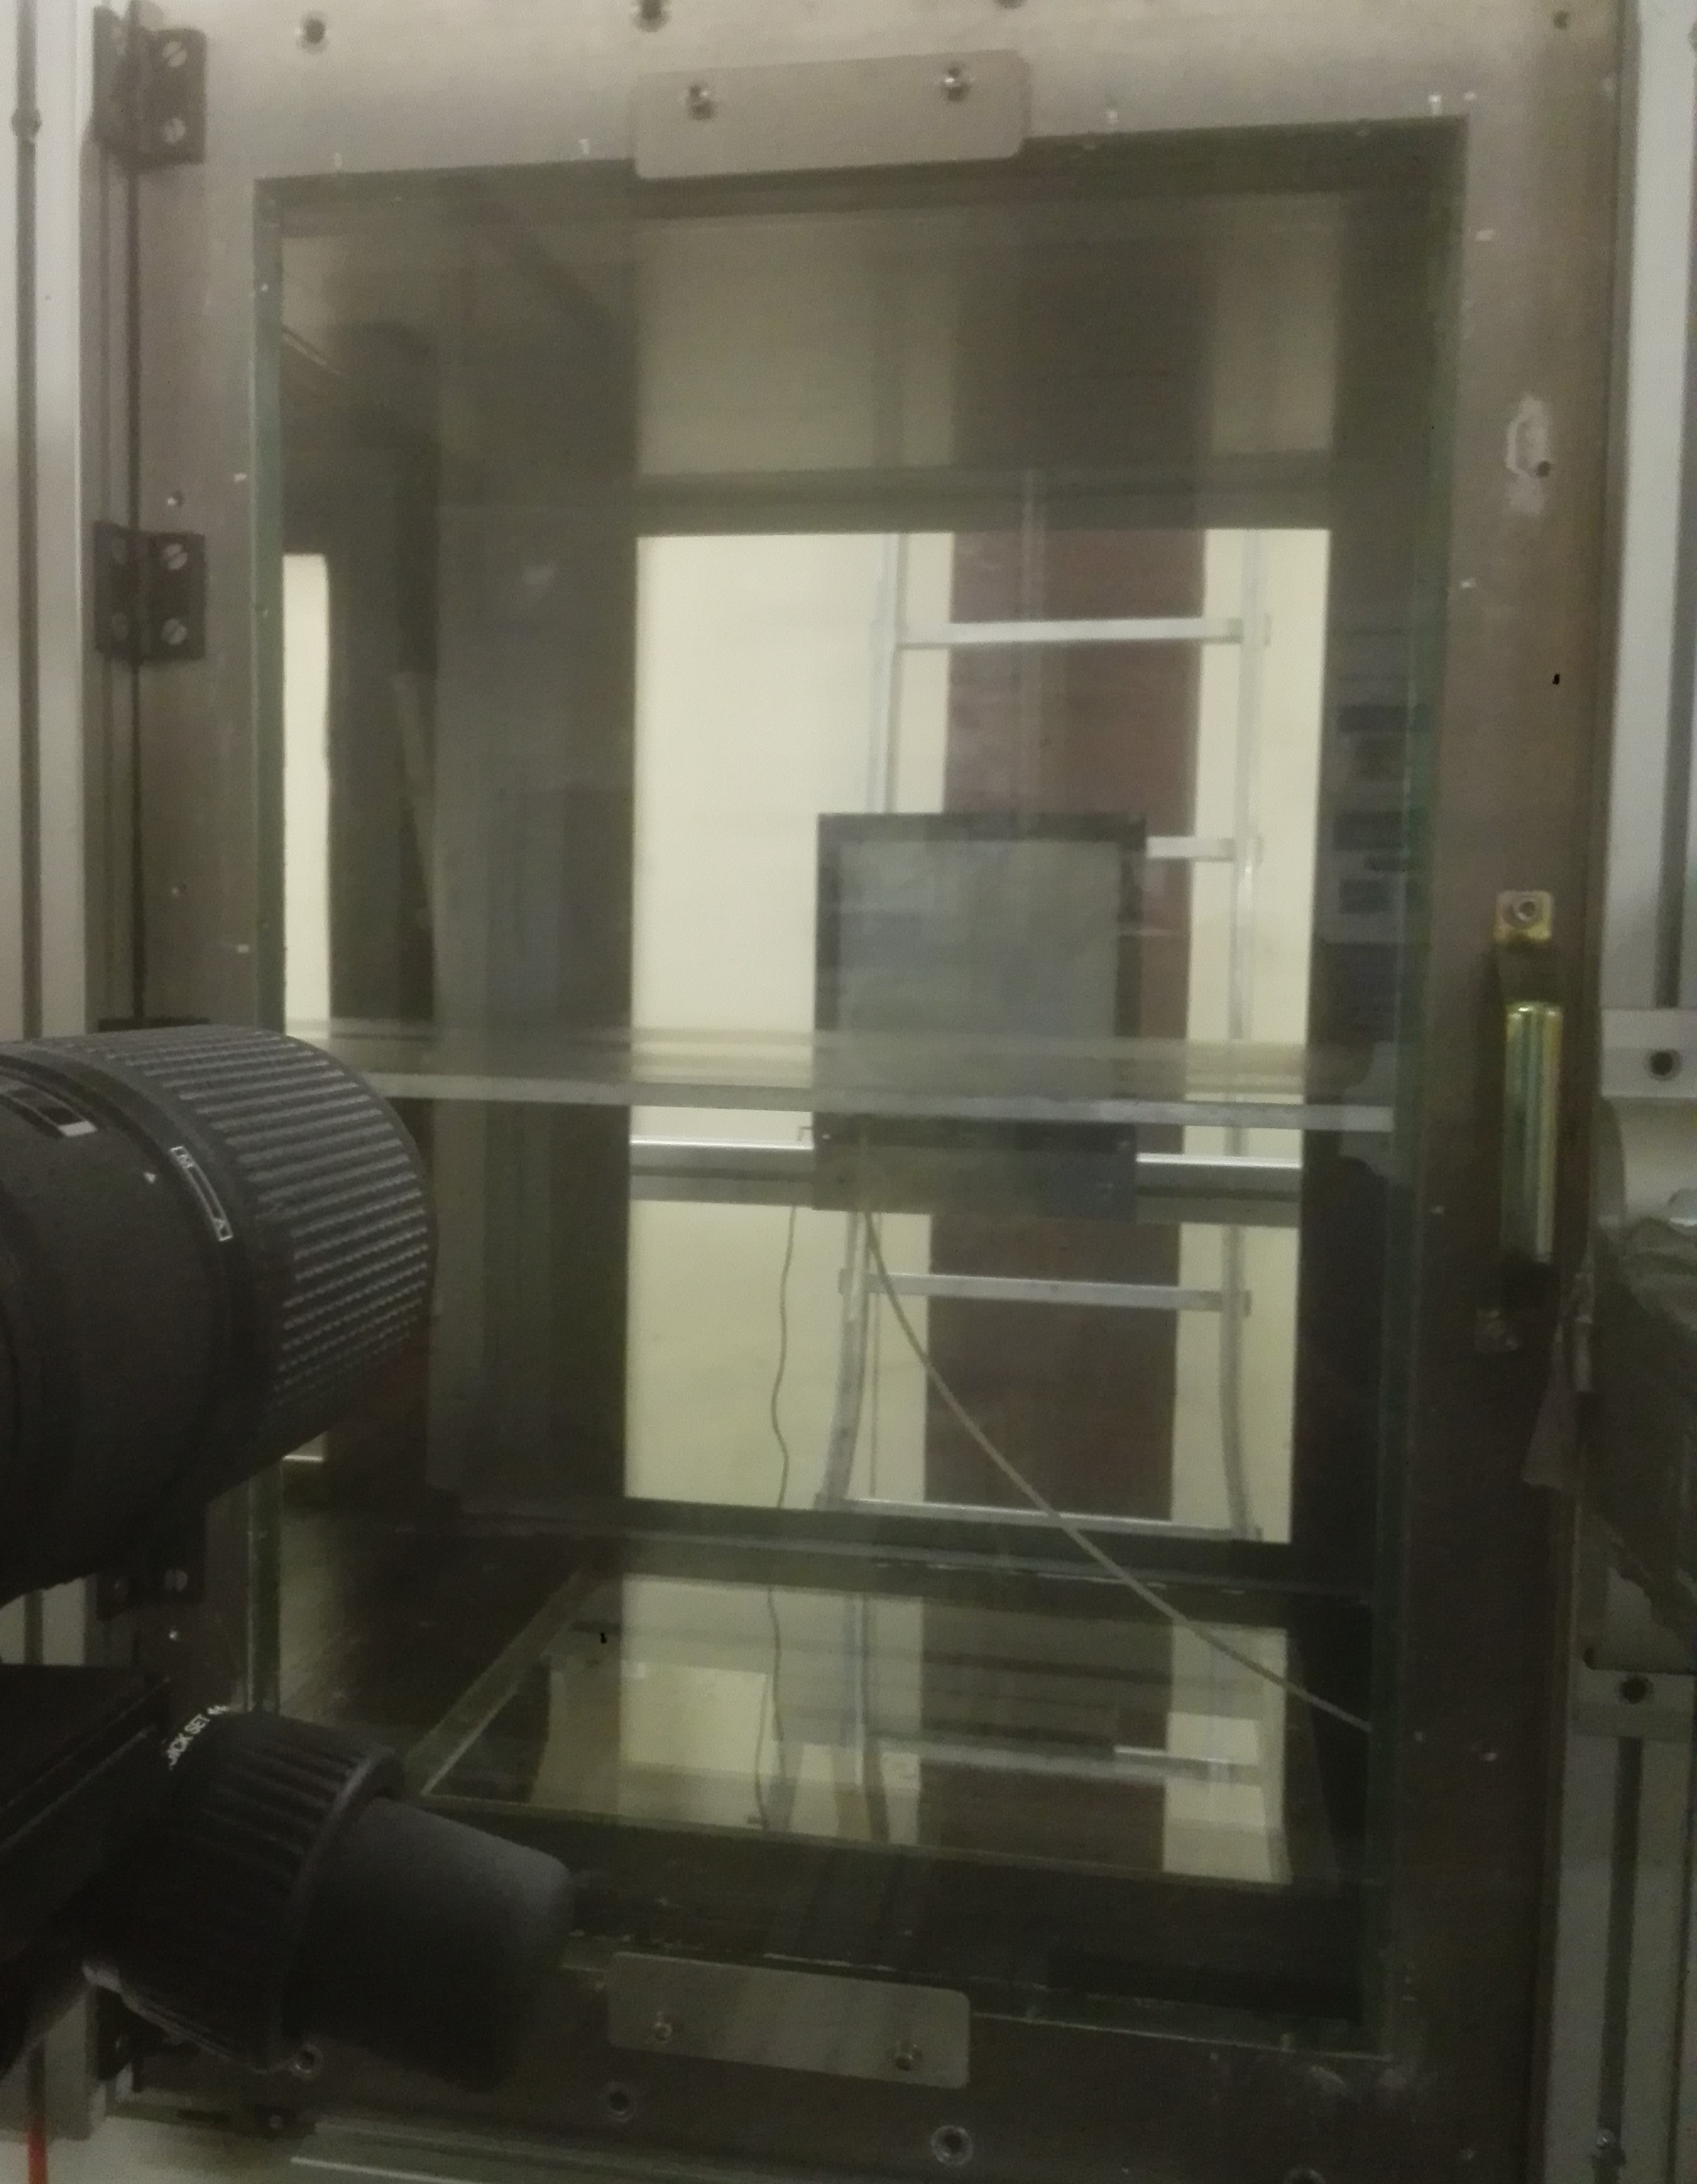
\includegraphics[width = 0.4\linewidth]{./image/Surface.jpg}
	\caption{Camera, surface et écran à laser}
	\label{fig:Plan}
\end{figure}
\begin{figure}[hb]
\centering
	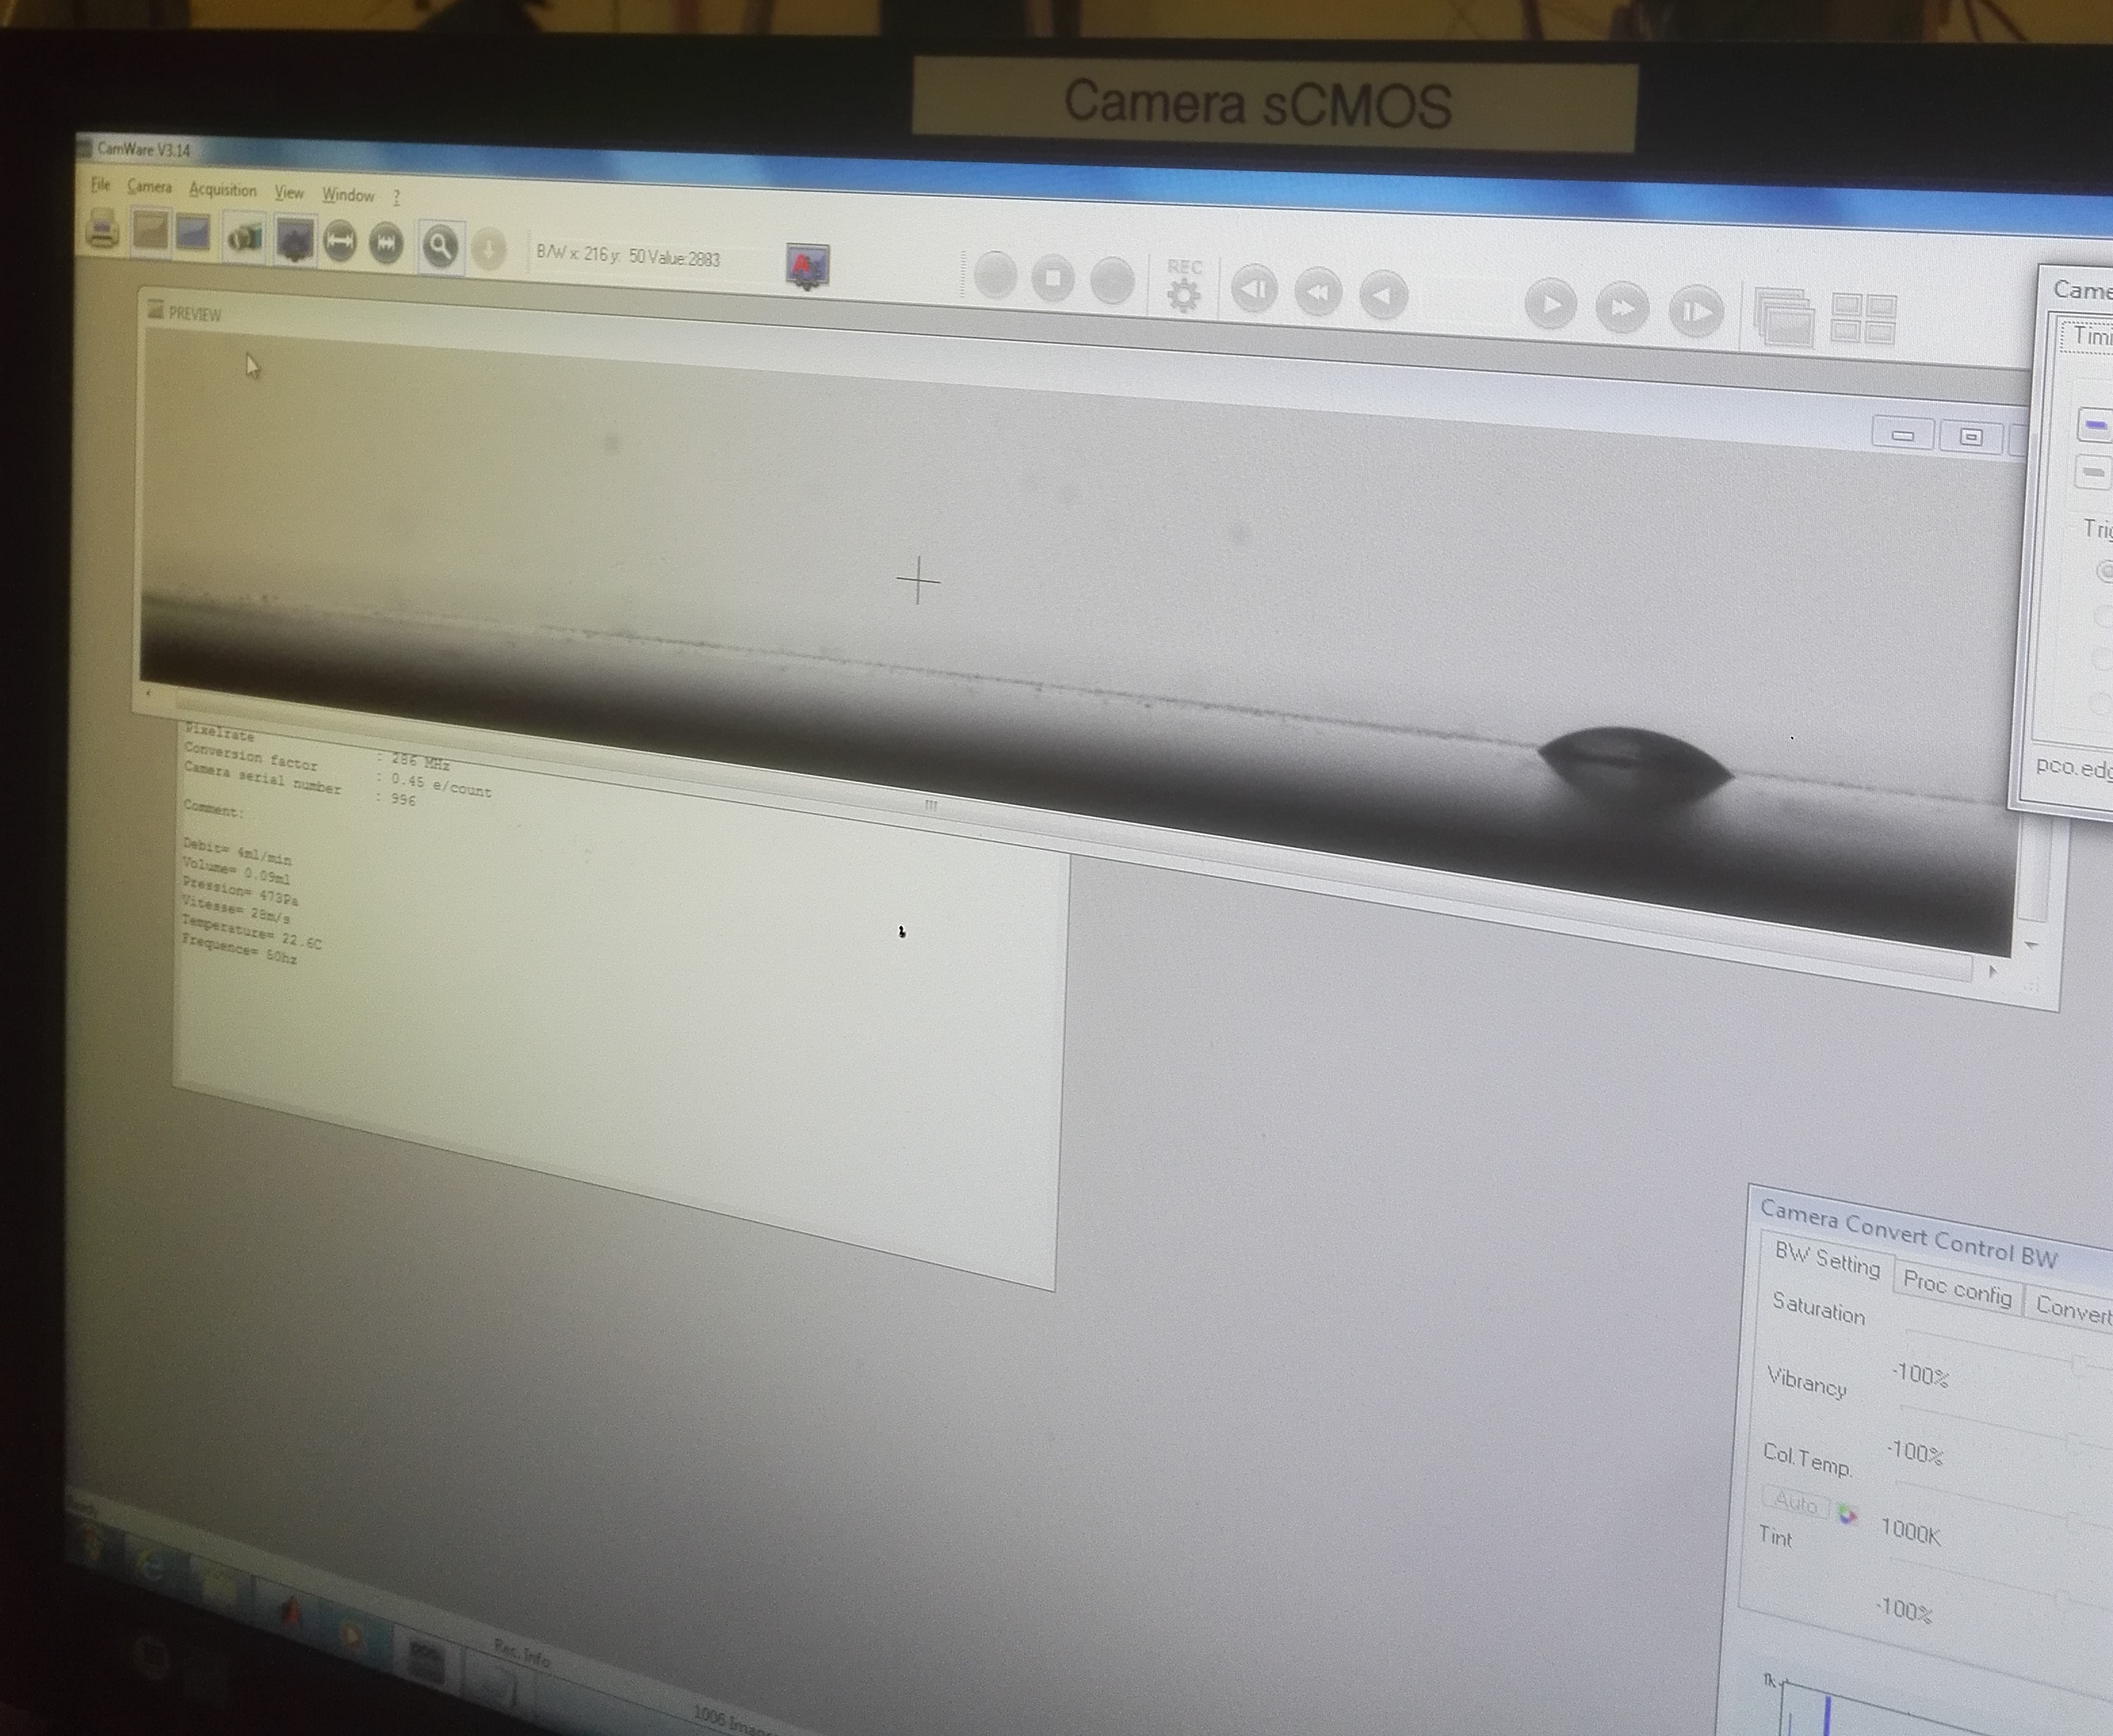
\includegraphics[width = 0.5\linewidth]{./image/Ecran.jpg}
	\caption{Ecran d'observation}
	\label{fig:Ecran d'observation}
\end{figure}

\newpage

\section{Anémomètre à fil chaud}
C'est l'anémomètre à fil chaud qui nous a permis de déterminer les profils de la couche limite dans notre écoulement.

Le principe de l'anénomètre à fil chaud est de placer un fil chaud (de l'ordre de $1mm$ de long et de $1\mu m$ de diamètre) dans l'écoulement et de maintenir sa température constante.

l'écoulement retirera une énergie au fil chaud et pour maintenir la température constante du fil chaud, on lui fournit une certaine énergie et cette énergie fournie (la tension qu'il a fallu fournir) est liée à la vitesse au niveau du fil chaud.


\section{Paramètres mesurés}

\begin{figure}[ht]
	\centering
	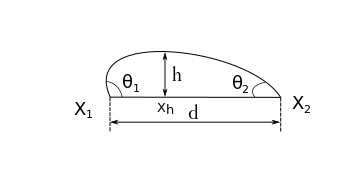
\includegraphics[scale = 1]{./image/rrgou2.png}
	\caption{Paramètres mesurés}
\end{figure}
\begin{figure}[ht]
	\centering
	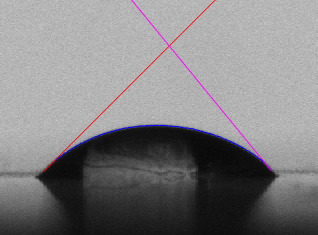
\includegraphics[scale = 0.5]{./image/crop_tvitesse=28_volume=003.png}
	\caption{Goutte d'eau de volume $0.03$ml avec $U = 0$, $\theta_{a} = \ang{45}$, $\theta_{r} = \ang{50.17}$, $x_{1} = 14.66mm$, $x_{2} = 6.77mm$, $d = 7.89mm$, $h = $ et $x_{h} = 4.86mm$}
\end{figure}


L'objectif du stage était de réussir à ressortir la courbe du contour d'une goutte à partir des photos prises avec notre caméra à la fréquence de $50hz$ et de pouvoir extraire les paramètres comme les angles de contact, la position avant et arrière de la goutte ou la hauteur maximale de la goutte et la position où on obtient cette hauteur maximale.

\newpage
\section{Mesures numériques}

Nous avons déterminé le contour de la goutte à l'aide de la fonction de Matlab \emph{bwboundaries} qui nous donnait (après avoir réussi à faire les ajustements pour cibler notre zone d'intérêt) le contour sous forme de nuage points.

Ce fut une étape assez difficile dont on a trouvé une solution qui nous satisfaisait assez tardivement (avoir le contour et la positions des points extrêmes ($x_{1}$ et $x_{2}$) ont posé beaucoup de difficulté).  \\

Une fois le nuage de points de définissant le contour ayant été obtenu, obtenir les tangentes aux deux extrémités de la goutte nous a aussi pris assez de temps.

Nous avons essayé de trouver des courbes d'interpolation autour de chaque extrémité (les points dont nous voulions les tangentes), mais les différentes fonctions d'interpolation de Matlab ou nos différentes méthodes n'arrivaient pas être visuellement proche de la tangente attendue lorsque la goutte changeait de forme.\\

Nos gouttes prenaient des formes plus proche d'une courbe paramétrée en coordonnées polaires comme un cardioïde, les formes des gouttes étaient aussi souvent proche des coniques et les méthodes d'interpolation, en particulier celle se basant sur la recherche des polynômes d'ordre 2 ou plus, s'éloignaient très souvent des tangentes attendues visuellement.\\

C'est l'interpolation par un polynôme d'ordre 1 qui donnait des résultats toujours proche des tangentes qu'on pouvait s'attendre visuellement, mais le nombre de points pris pour déterminer notre tangente avec la fonction \emph{polyfit} de Matlab jouait un rôle important.

Sur un cas particulier, nous pouvions ajuster le nombre de points pour avoir une meilleure tangente (visuellement).

Notre difficulté était de faire un algorithme pour traiter des milliers d'images qui arrivent à ajuster le nombre de points.

Nous partions de $n$ points (le maximum entre 2 et $1\%$ du nombre de points dans notre nuage de points) puis nous trouvions les tangentes avec $n$ et $n+1$.

Si les tangentes avec $n$ et $n+1$ faisaient entre elles un angle inférieure à $\ang{0.5}$, nous conservions la tangente faite avec $n$ points, sinon on posait $n = n+1$ et on recommençait.

Si nous n'arrivions pas à avoir un angle inférieur à \ang{0.5}  entre les tangentes avec $n$ points et avec $n+1$ points, nous ne conservions pas l'image dans nos résultats faute de ne pouvoir avoir les angles de contact assez précisément.

\newpage
\section{Mesures expérimentales}

Nos mesures dans la soufflerie ont été effectuées de 2 manières.\\

D'abord, nous mettions d'abord en marche la soufflerie jusqu'à ce que la vitesse se stabilise puis on un on injectait le volume de goutte désirée.

La difficuté de cette méthode est que la goutte d'eau se mettait souvent en mouvement avant la fin d'injection, avant d'atteindre le volume de goutte d'eau désirée.\\

Ensuite nous injections d'abord la goutte d'eau de volume désiré et c'est par la suite que nous mettions la soufferie en marche.

Dans ce cas la vitesse de la soufflerie prends relativement court à se stabiliser donc nous n'avons pas la vitesse désirée toute suite.\\

C'est dernière méthode où le débit n'était pas un paramètre important que présenterons davantage les résultats et nous ferons un comparatif lorsque le début jouait un rôle important.

\newpage
\section{Résultat}

Nous présentons les résultats obtenus après l'extraction de nos paramètres et nous en ferons une analyse.

\subsection{Angle de contact avant}
\begin{figure}[h]
	\centering
	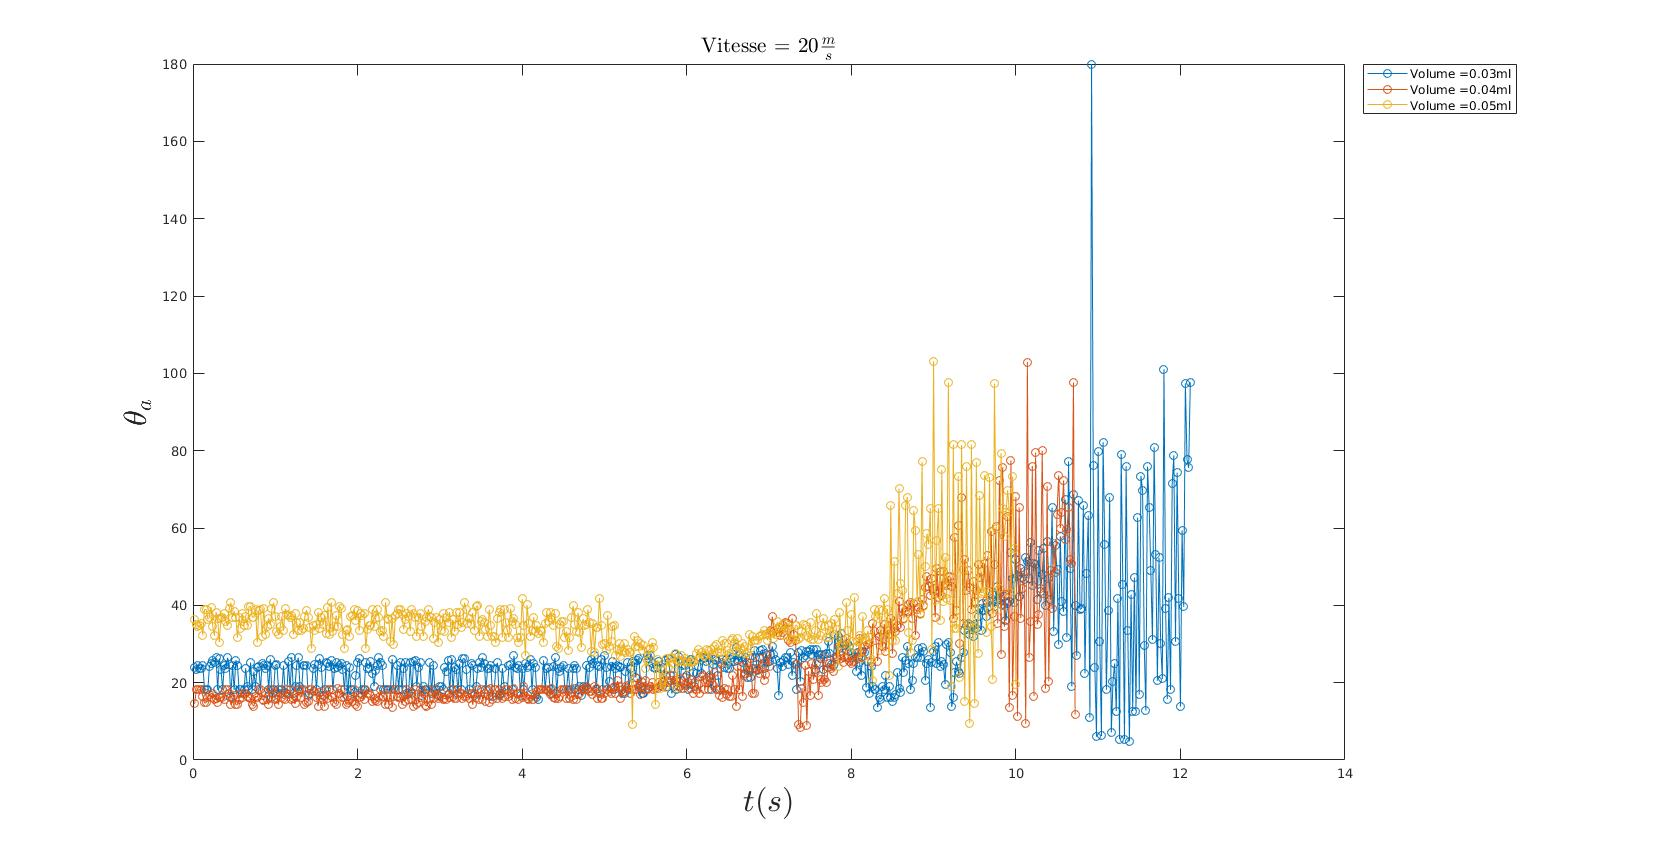
\includegraphics[width = \linewidth]{./image/v=20oa_1.jpg}
	\caption{Angle à l'avant pour une vitesse de $20m\mathbin{/}s$}
\end{figure}
\begin{figure}[h]
	\centering
	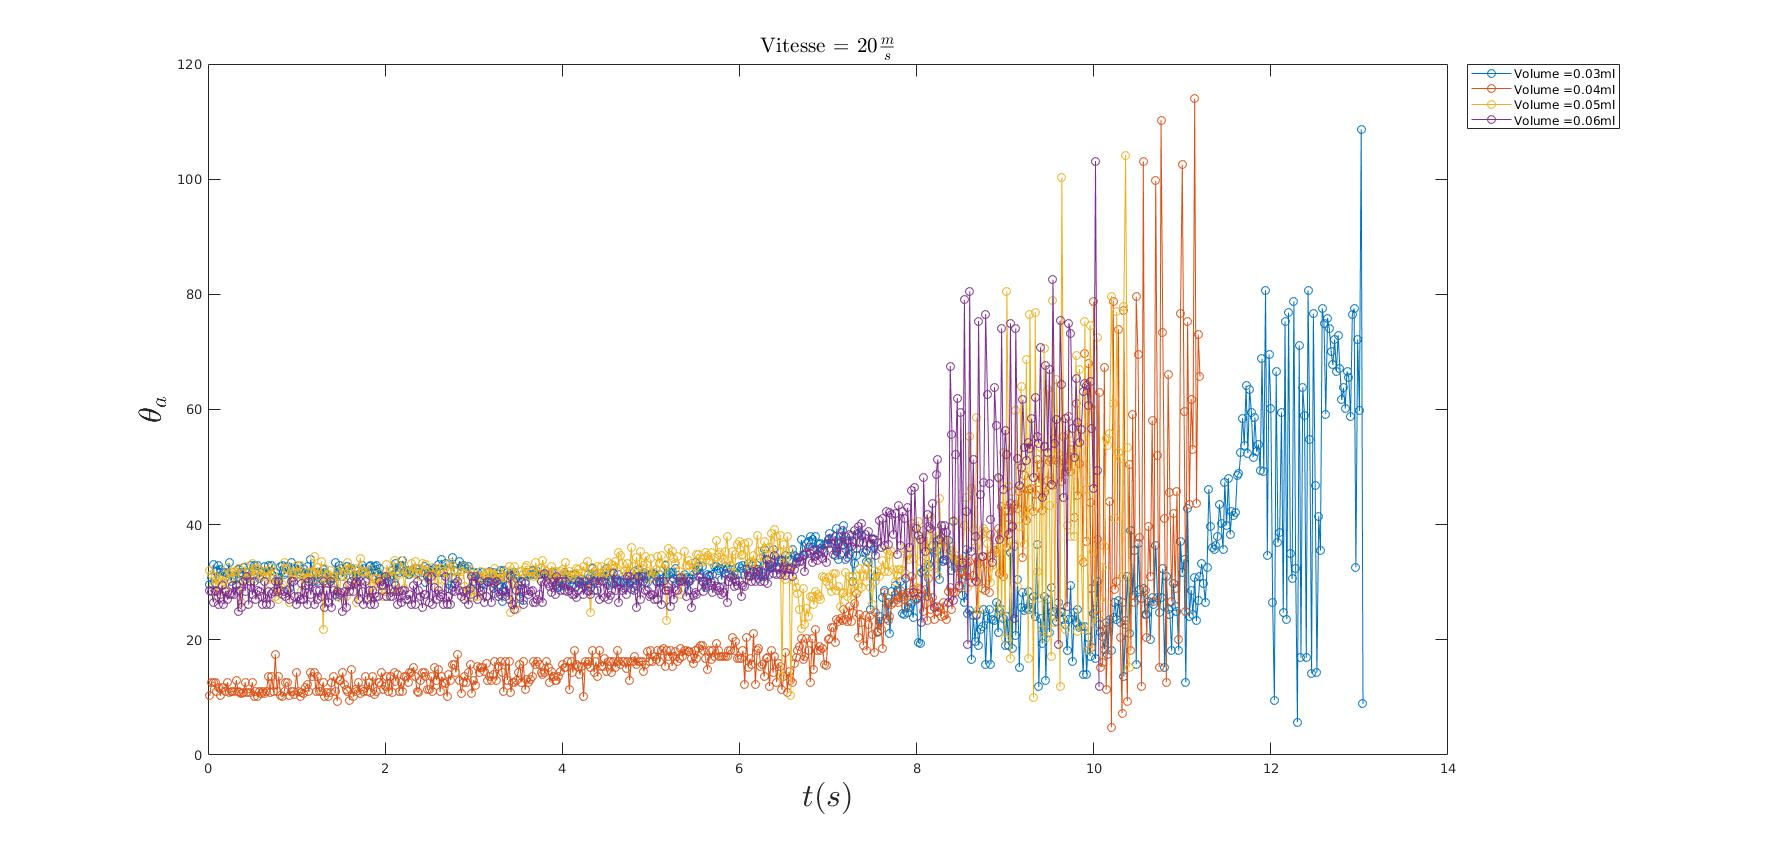
\includegraphics[width = \linewidth]{./image/v=20oa_2.jpg}
	\caption{Angle à l'avant pour une vitesse de $20m\mathbin{/}s$}
\end{figure}
\begin{figure}[h]
	\centering
	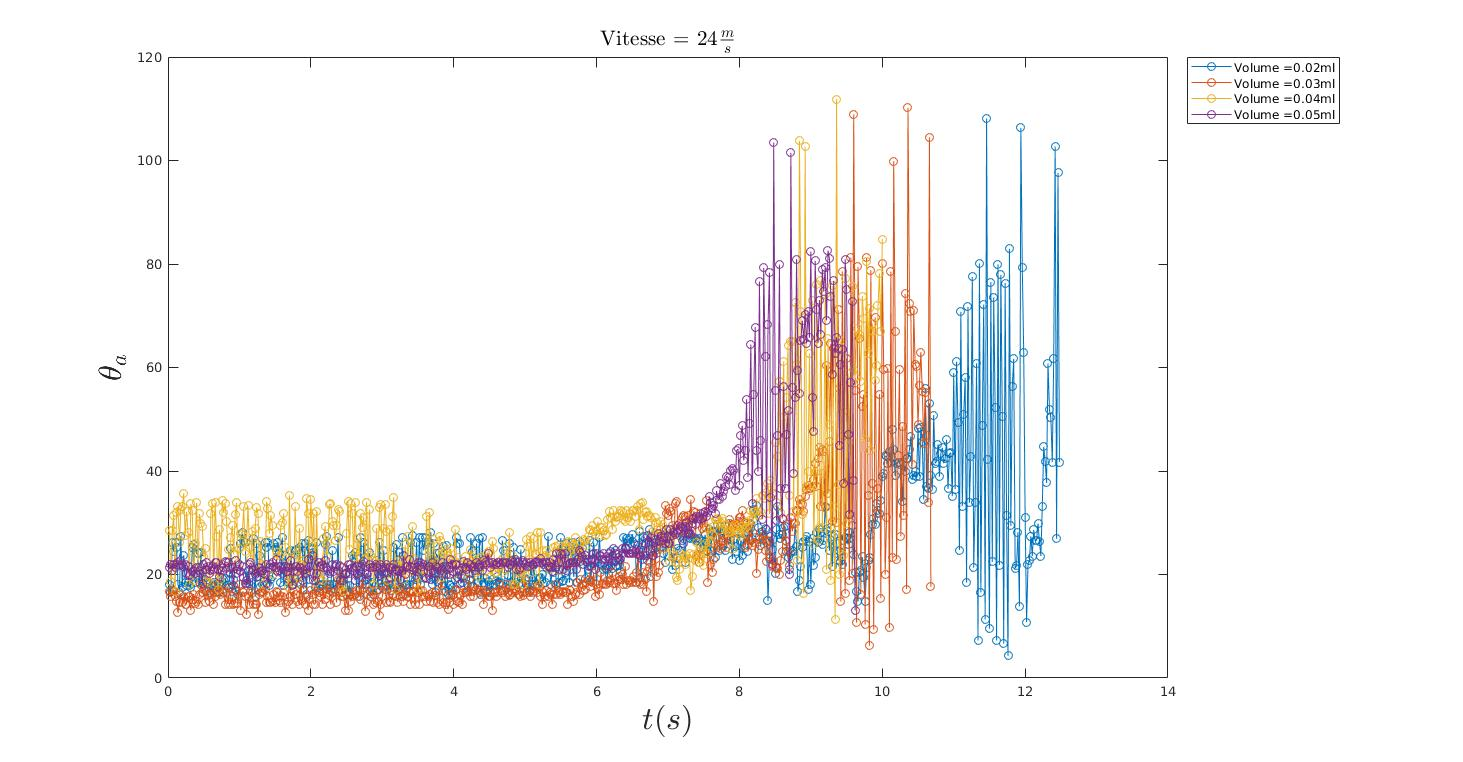
\includegraphics[width = \linewidth]{./image/v=24oa_1.jpg}
	\caption{Angle à l'avant pour une vitesse de $24m\mathbin{/}s$}
\end{figure}
\begin{figure}[h]
	\centering
	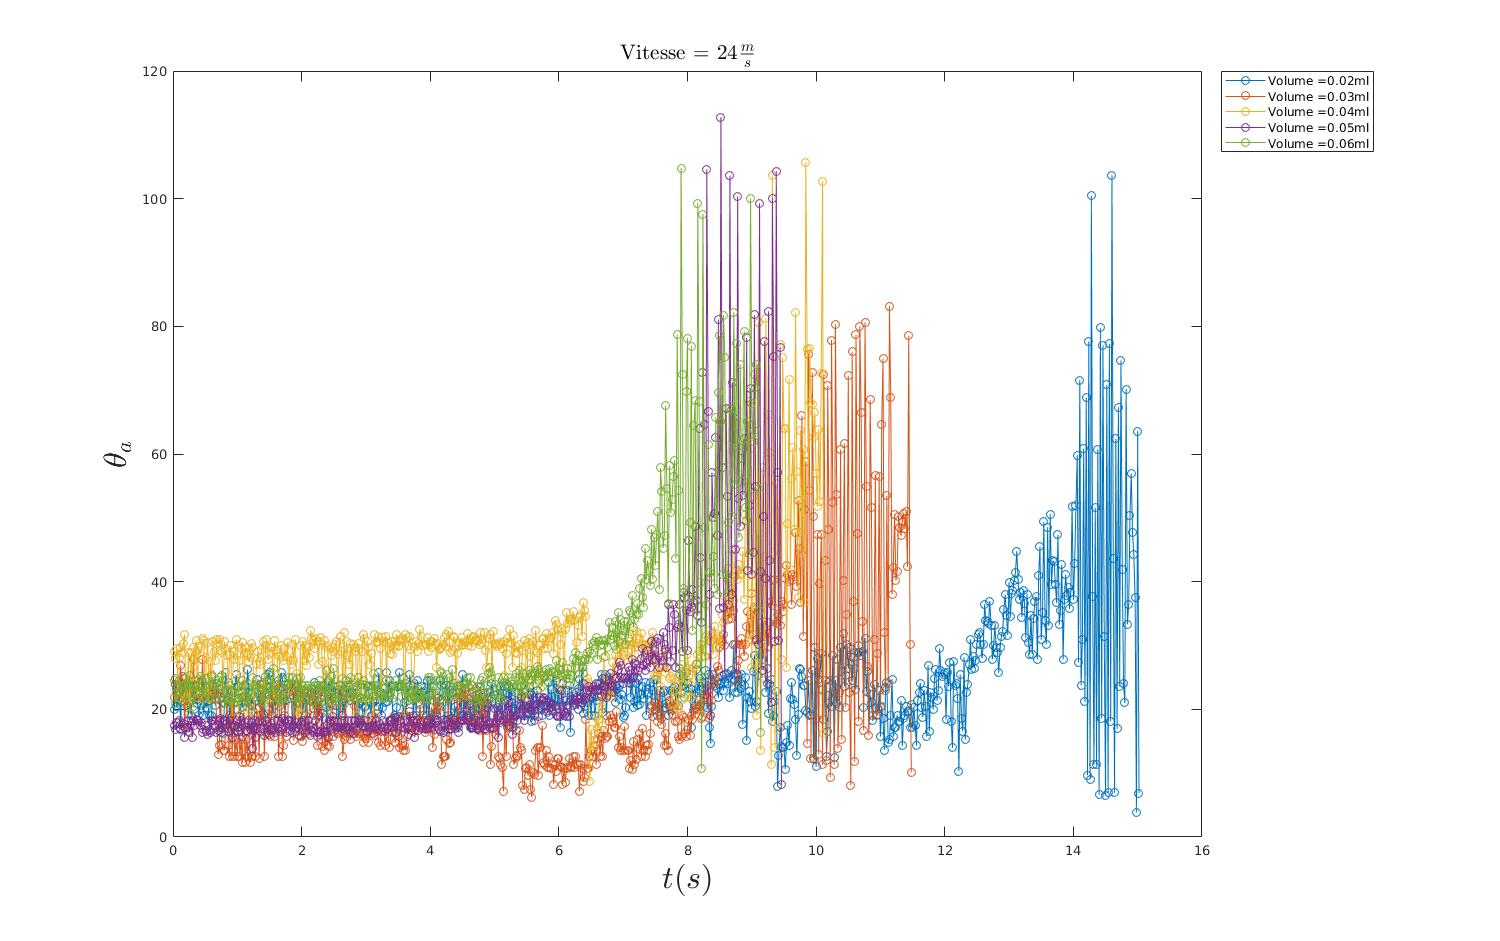
\includegraphics[width = \linewidth]{./image/v=24oa_2.jpg}
	\caption{Angle à l'avant pour une vitesse de $24m\mathbin{/}s$}
\end{figure}
\begin{figure}[h]
	\centering
	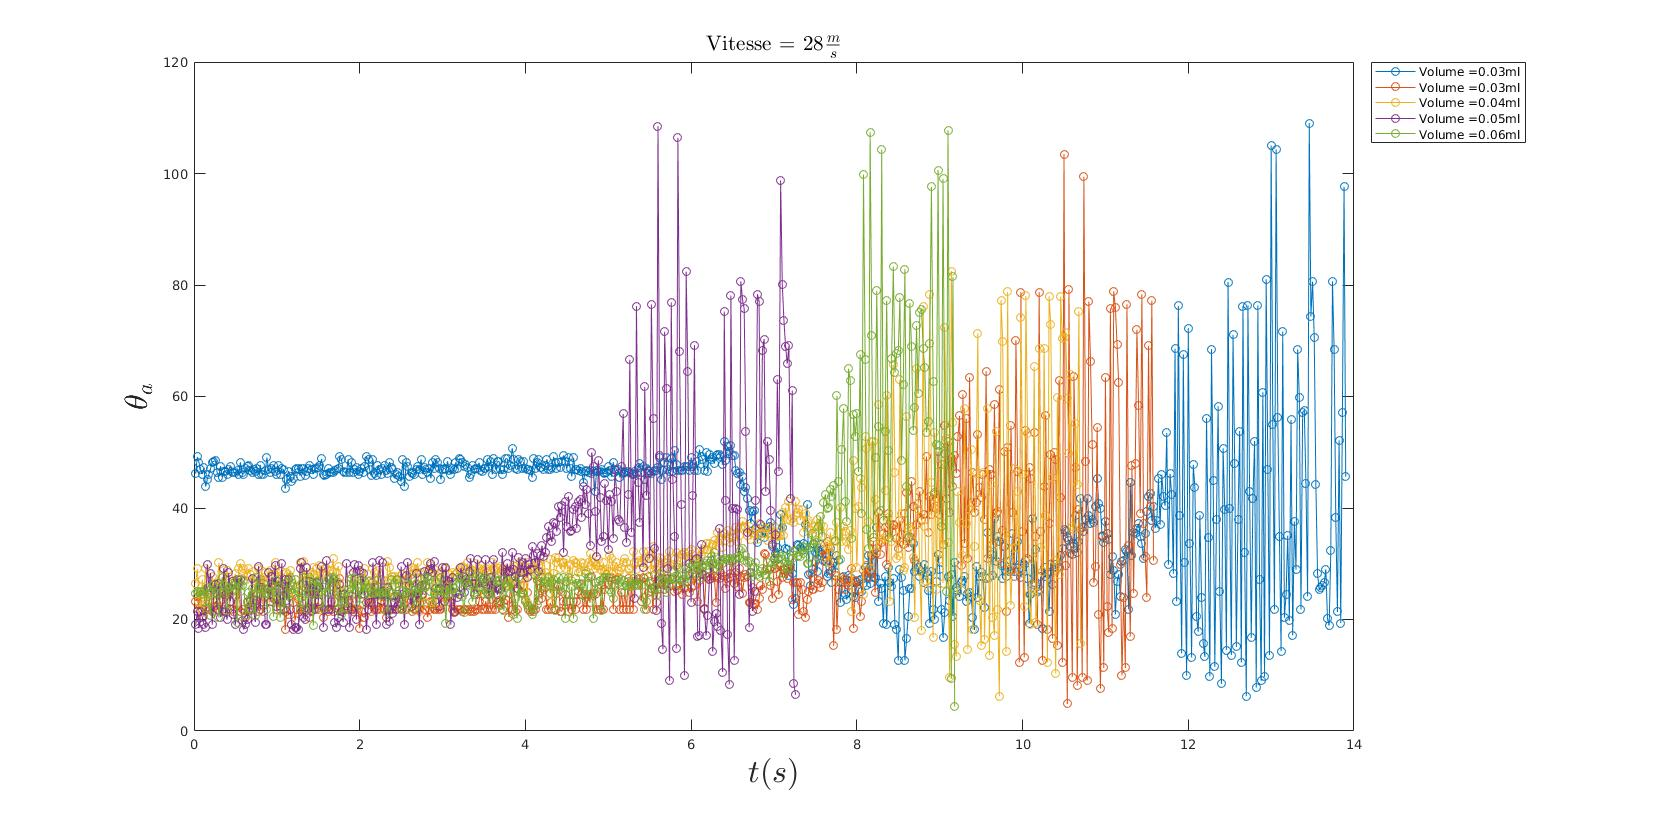
\includegraphics[width = \linewidth]{./image/v=28oa_1.jpg}
	\caption{Angle à l'avant pour une vitesse de $28m\mathbin{/}s$}
\end{figure}
\begin{figure}[h]
	\centering
	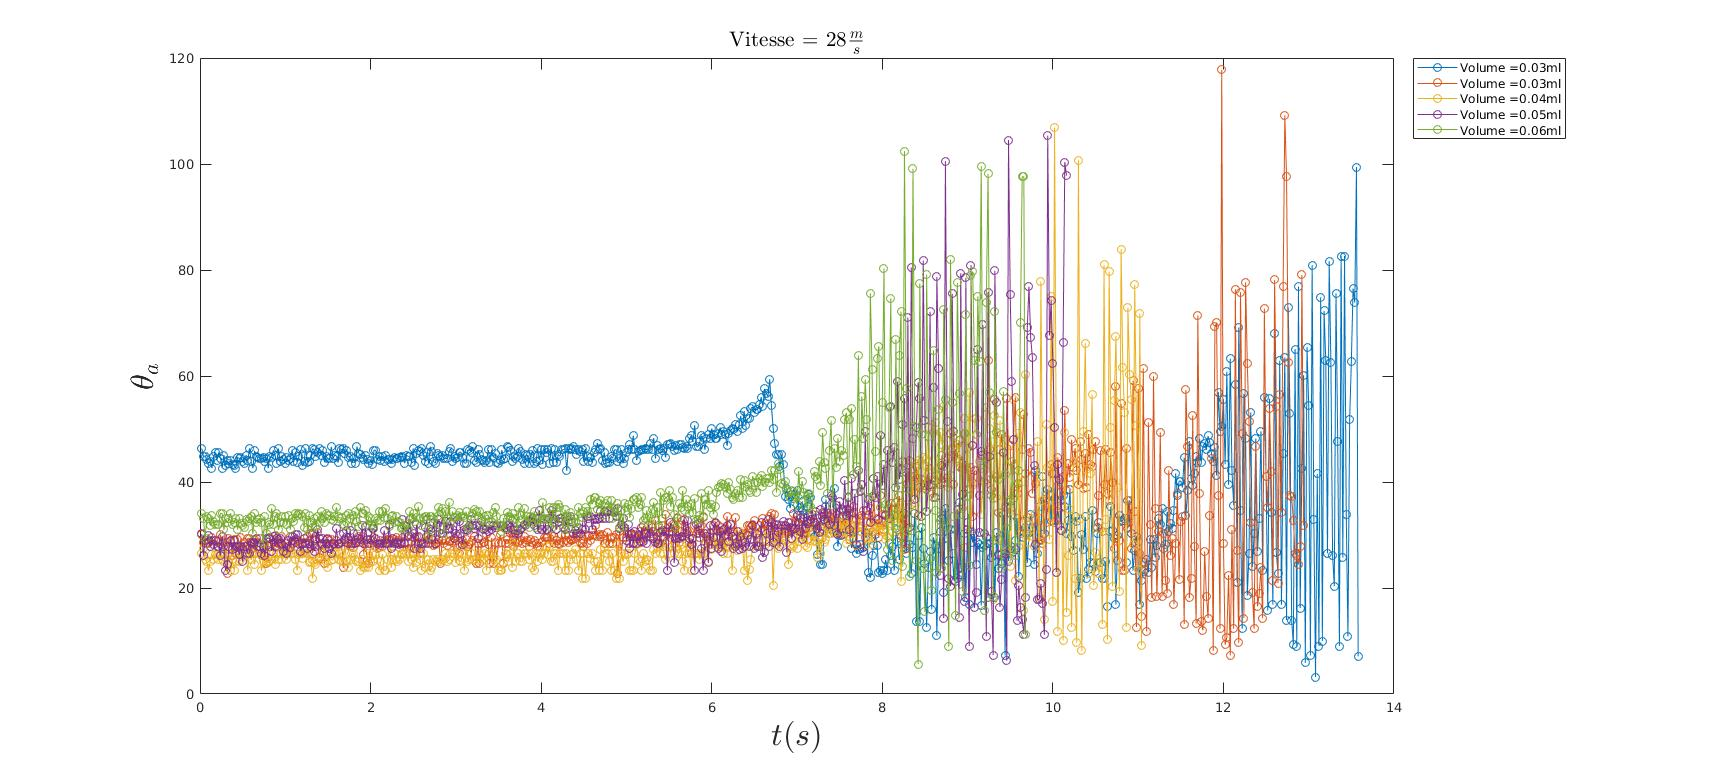
\includegraphics[width = \linewidth]{./image/v=28oa_2.jpg}
	\caption{Angle à l'avant pour une vitesse de $28m\mathbin{/}s$}
\end{figure}

Nous a avions pu constater dans nos expériences que l'angle d'avancé augmentait globalement au cours du temps, ce que semble indiqué les figures.\\

Il y avait aussi des oscillations rapides autour d'un certaine position avant que la goutte avance de nouveau (le point avant avançait puis reculait) avant d'avant et c'est que doit traduire cette oscillation d'angle tout en augmentant globalement.

\newpage
\subsection{Angle de contact arrière}
\begin{figure}[ht]
	\centering
	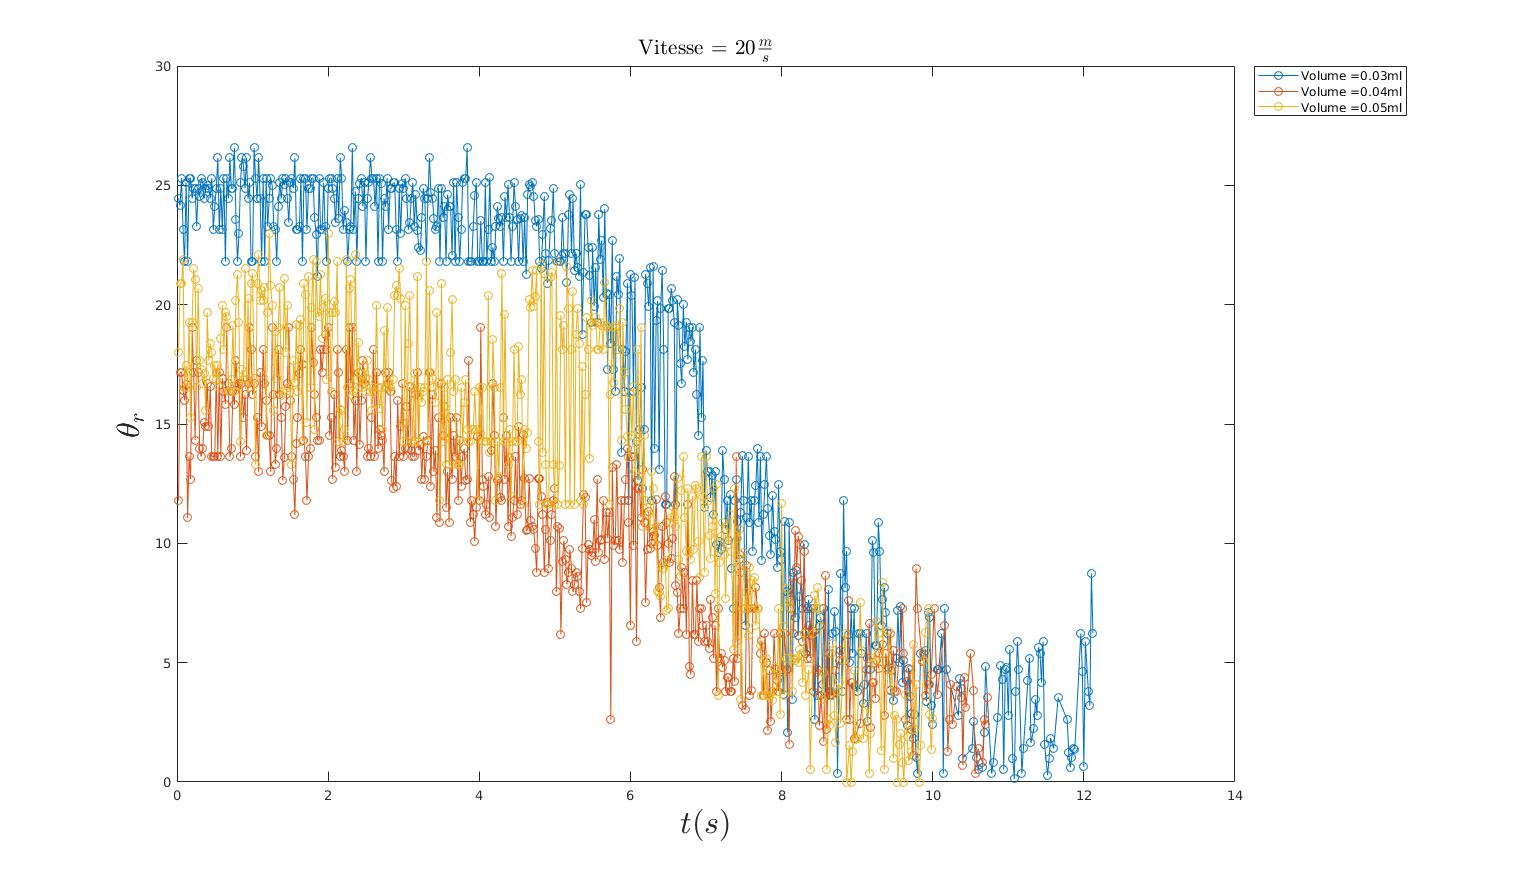
\includegraphics[width = \linewidth]{./image/v=20or_1.jpg}
	\caption{Angle à l'arrière pour une vitesse de $20m\mathbin{/}s$}
\end{figure}
\begin{figure}[ht]
	\centering
	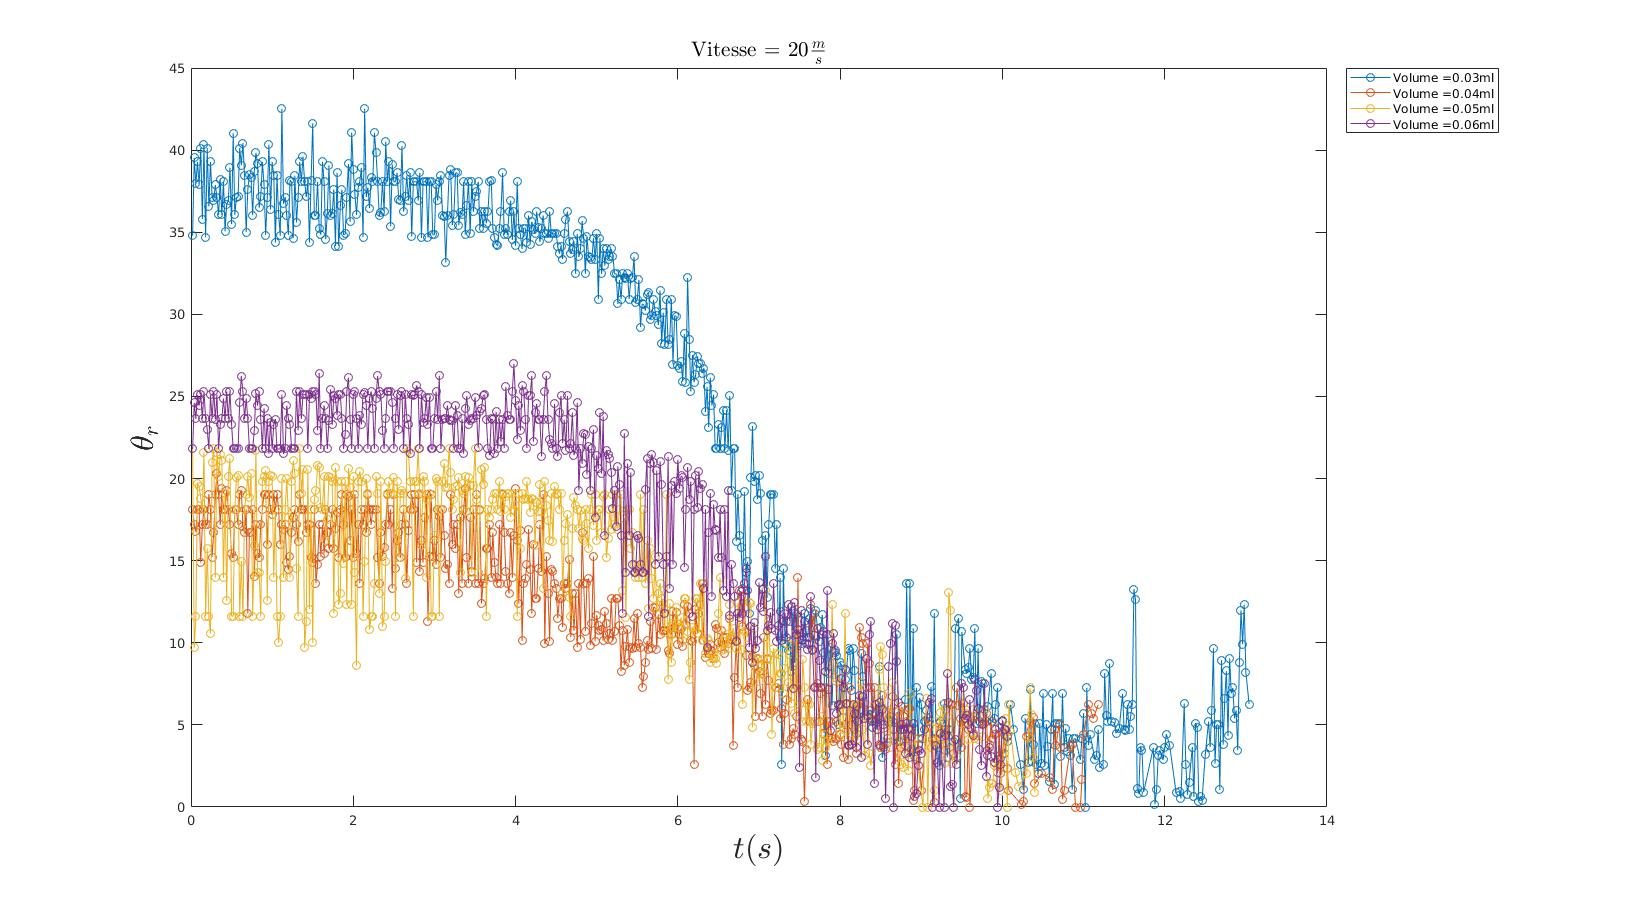
\includegraphics[width = \linewidth]{./image/v=20or_2.jpg}
	\caption{Angle à l'arrière pour une vitesse de $20m\mathbin{/}s$}
\end{figure}
\begin{figure}[h]
	\centering
	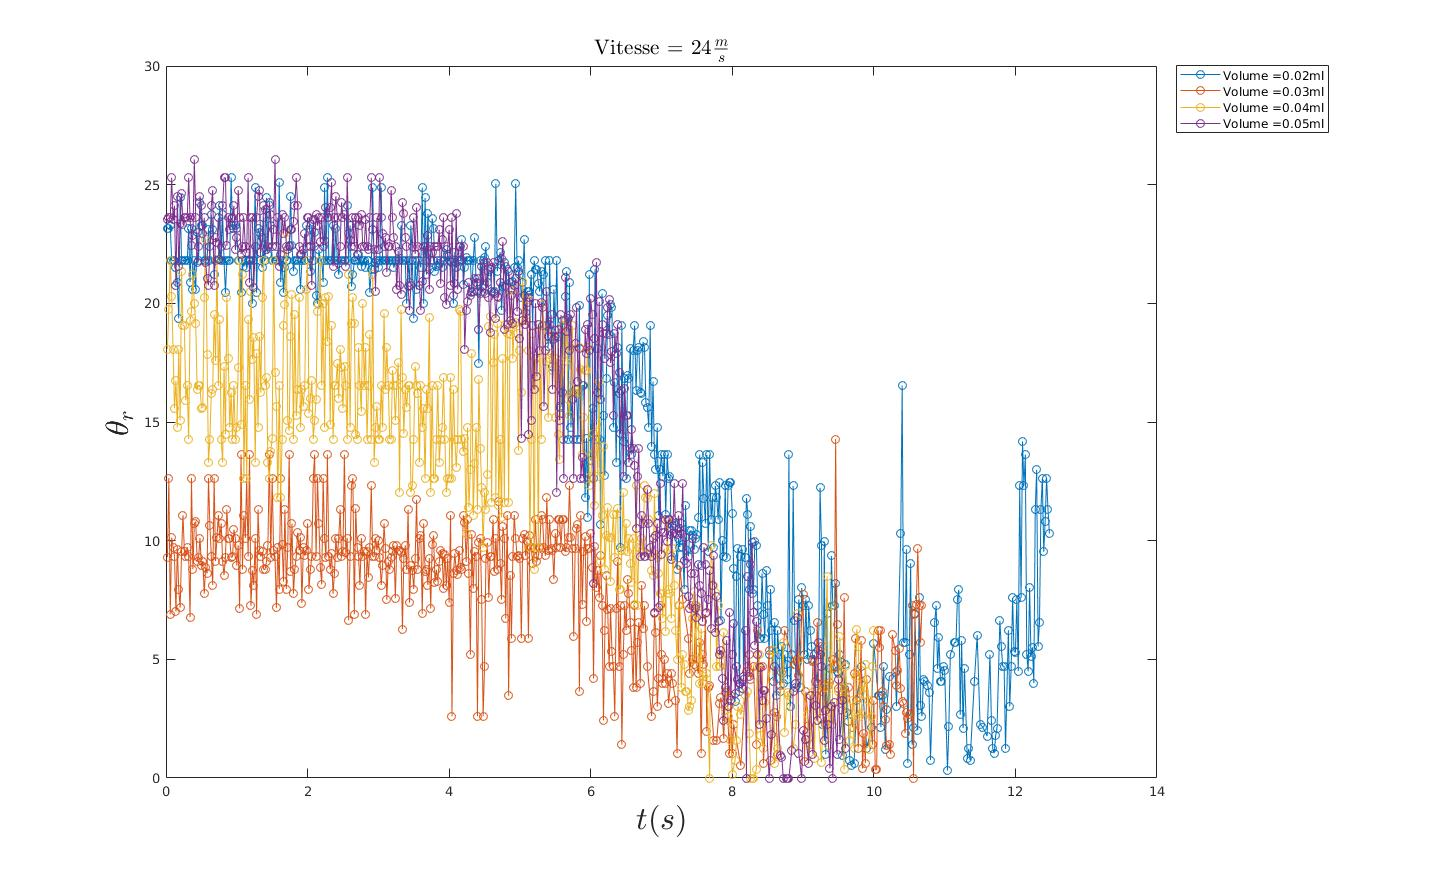
\includegraphics[width = \linewidth]{./image/v=24or_1.jpg}
	\caption{Angle à l'arrière pour une vitesse de $24m\mathbin{/}s$}
\end{figure}
\begin{figure}[hb]
	\centering
	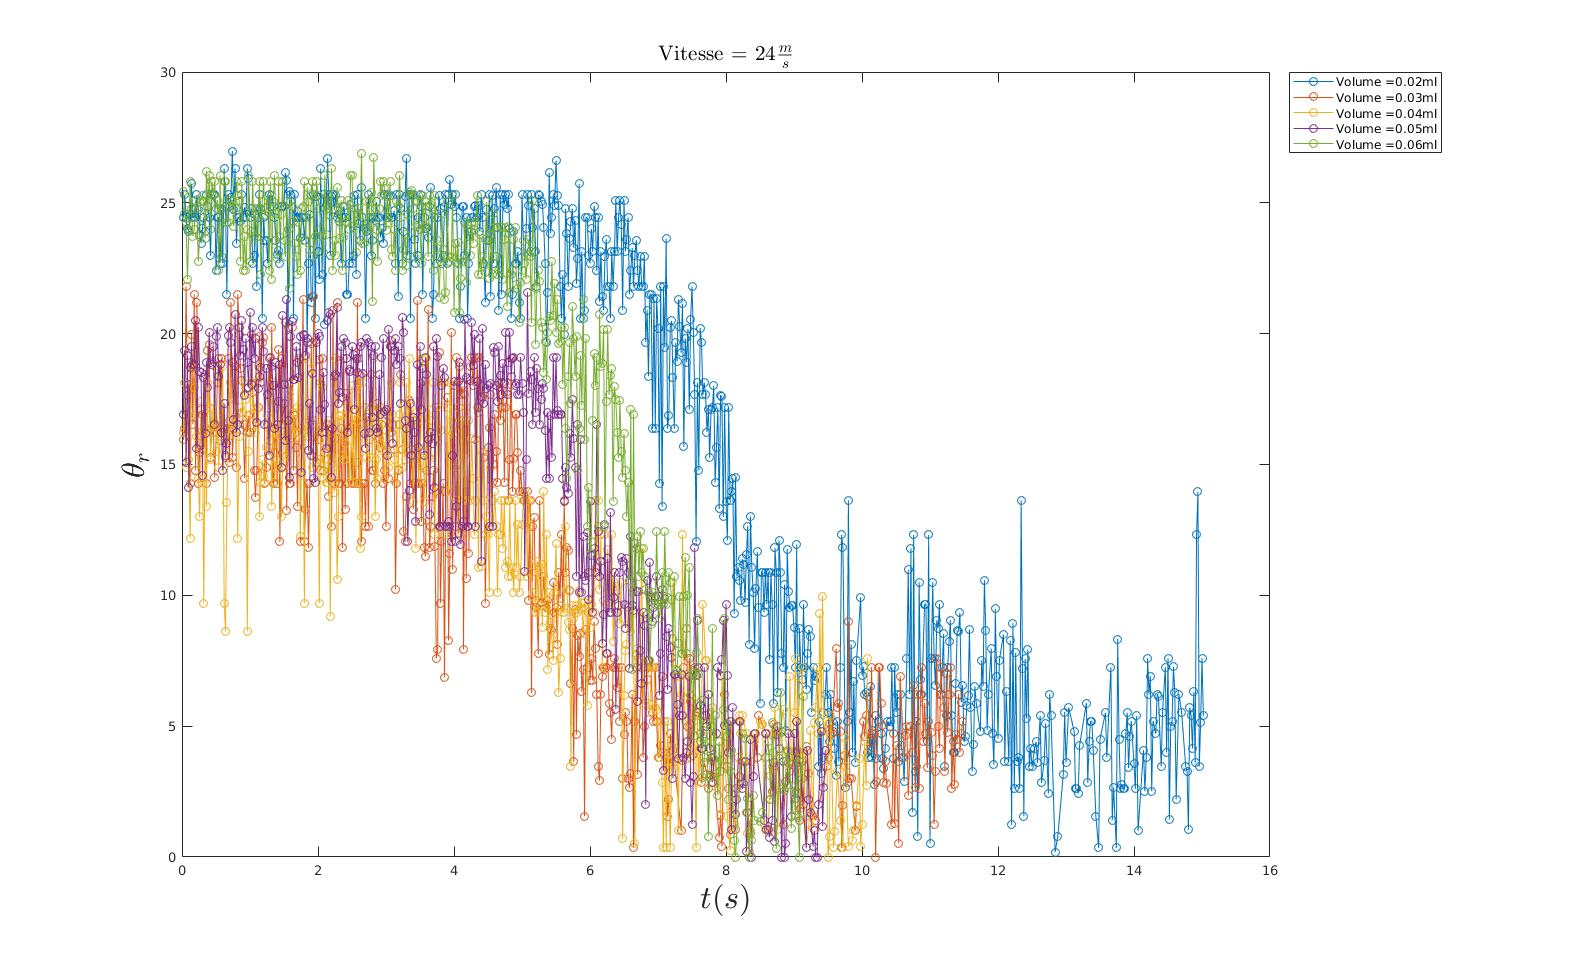
\includegraphics[width = \linewidth]{./image/v=24or_2.jpg}
	\caption{Angle à l'arrière pour une vitesse de $24m\mathbin{/}s$}
\end{figure}
\begin{figure}[hb]
	\centering
	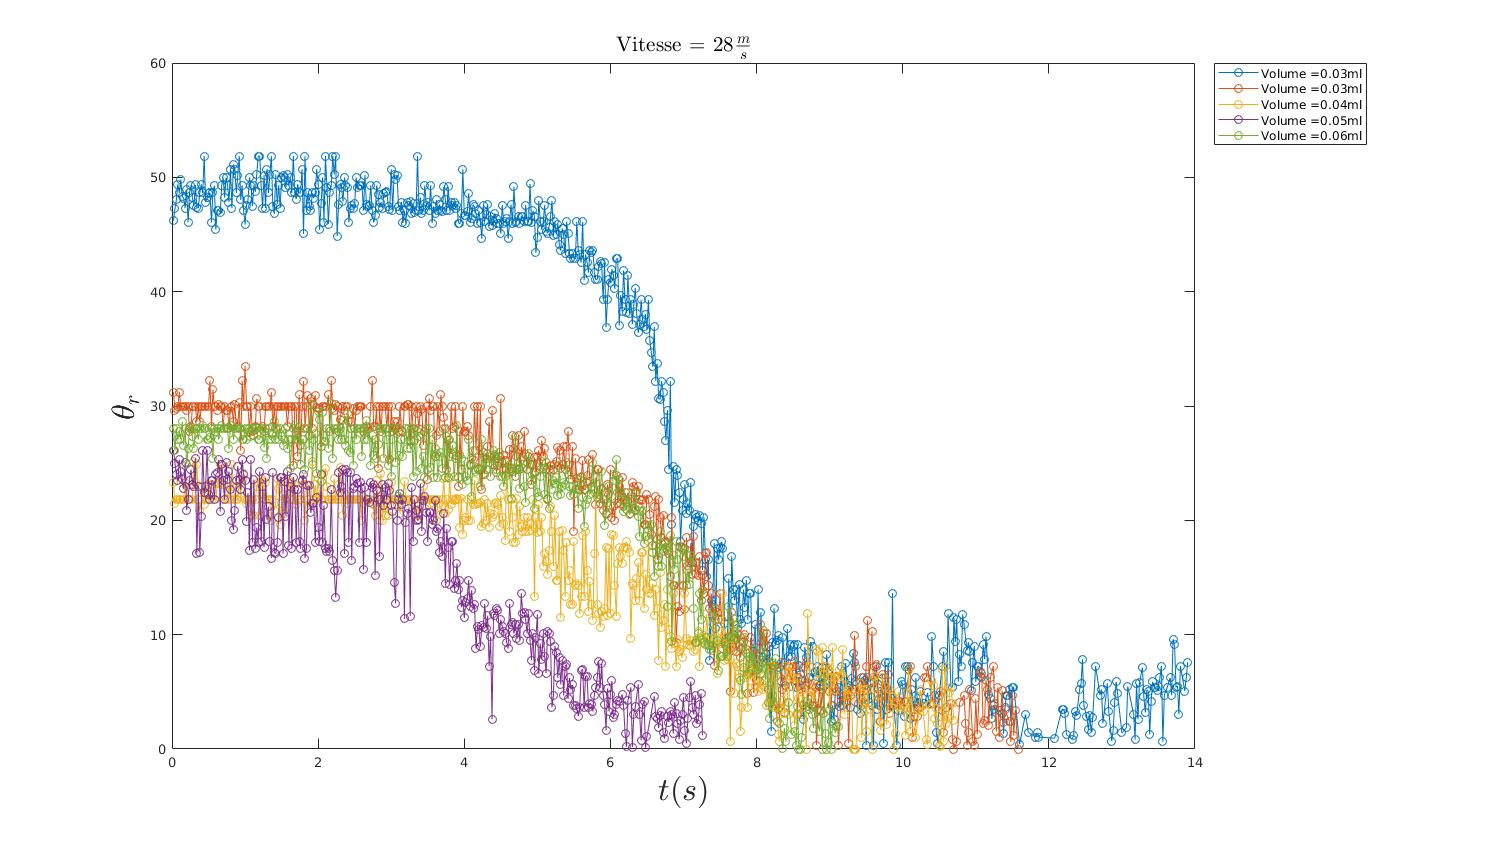
\includegraphics[width = \linewidth]{./image/v=28or_1.jpg}
	\caption{Angle à l'arrière pour une vitesse de $28m\mathbin{/}s$}
\end{figure}
\begin{figure}[h]
	\centering
	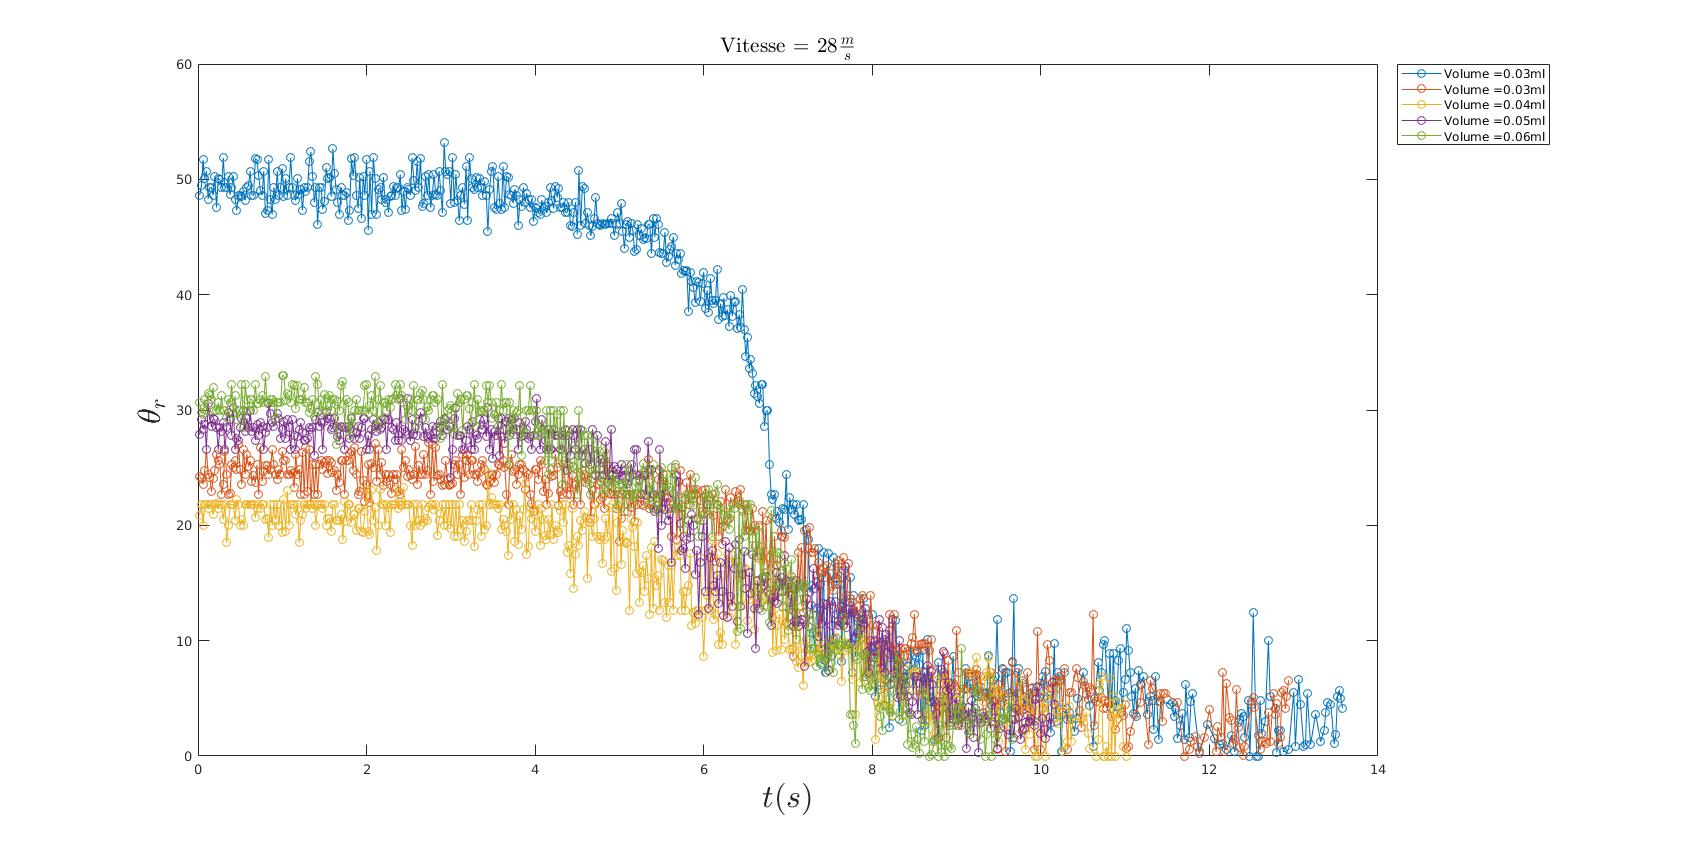
\includegraphics[width = \linewidth]{./image/v=28or_2.jpg}
	\caption{Angle à l'arrière pour une vitesse de $28m\mathbin{/}s$}
\end{figure}

\newpage
\subsection{Position de l'avant}
Nous a avions pu constater dans nos expériences que l'angle d'avancé augmentait globalement au cours du temps, ce que semble indiqué les figures.\\

Il y avait aussi des oscillations rapides autour d'un certaine position arrière que la goutte avance de nouveau (le point arrière avançait puis reculait) arrière d'arrière et c'est que doit traduire cette oscillation d'angle tout en augmentant globalement.

\begin{figure}[h]
	\centering
	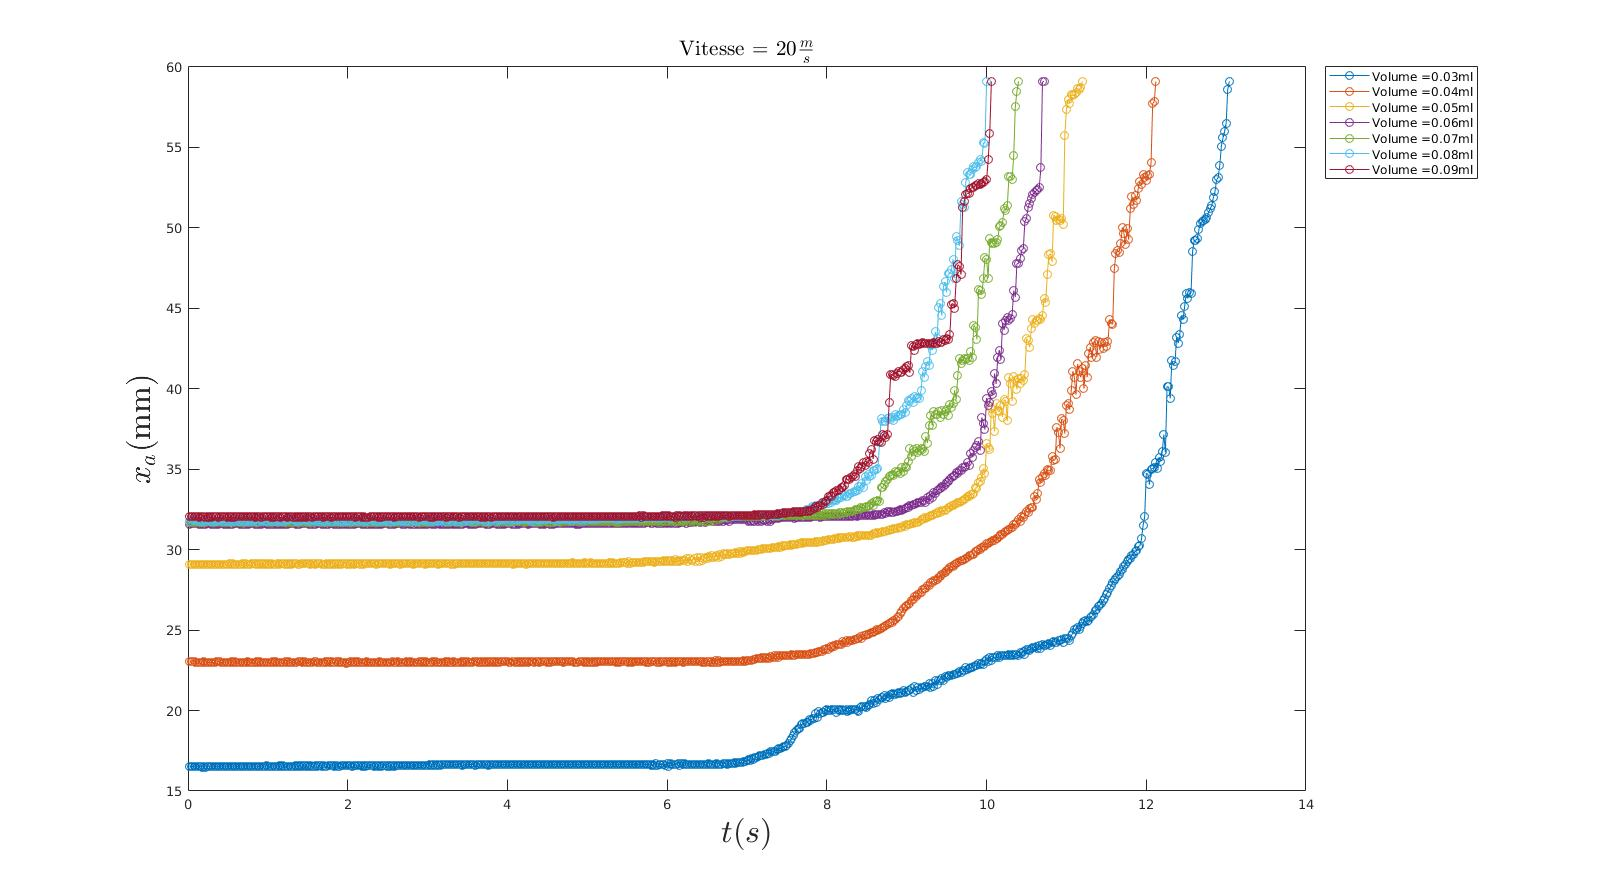
\includegraphics[width = \linewidth]{./image/v=20xa.jpg}
	\caption{Position à l'avant pour une vitesse de $20m\mathbin{/}s$}
\end{figure}
\begin{figure}[h]
	\centering
	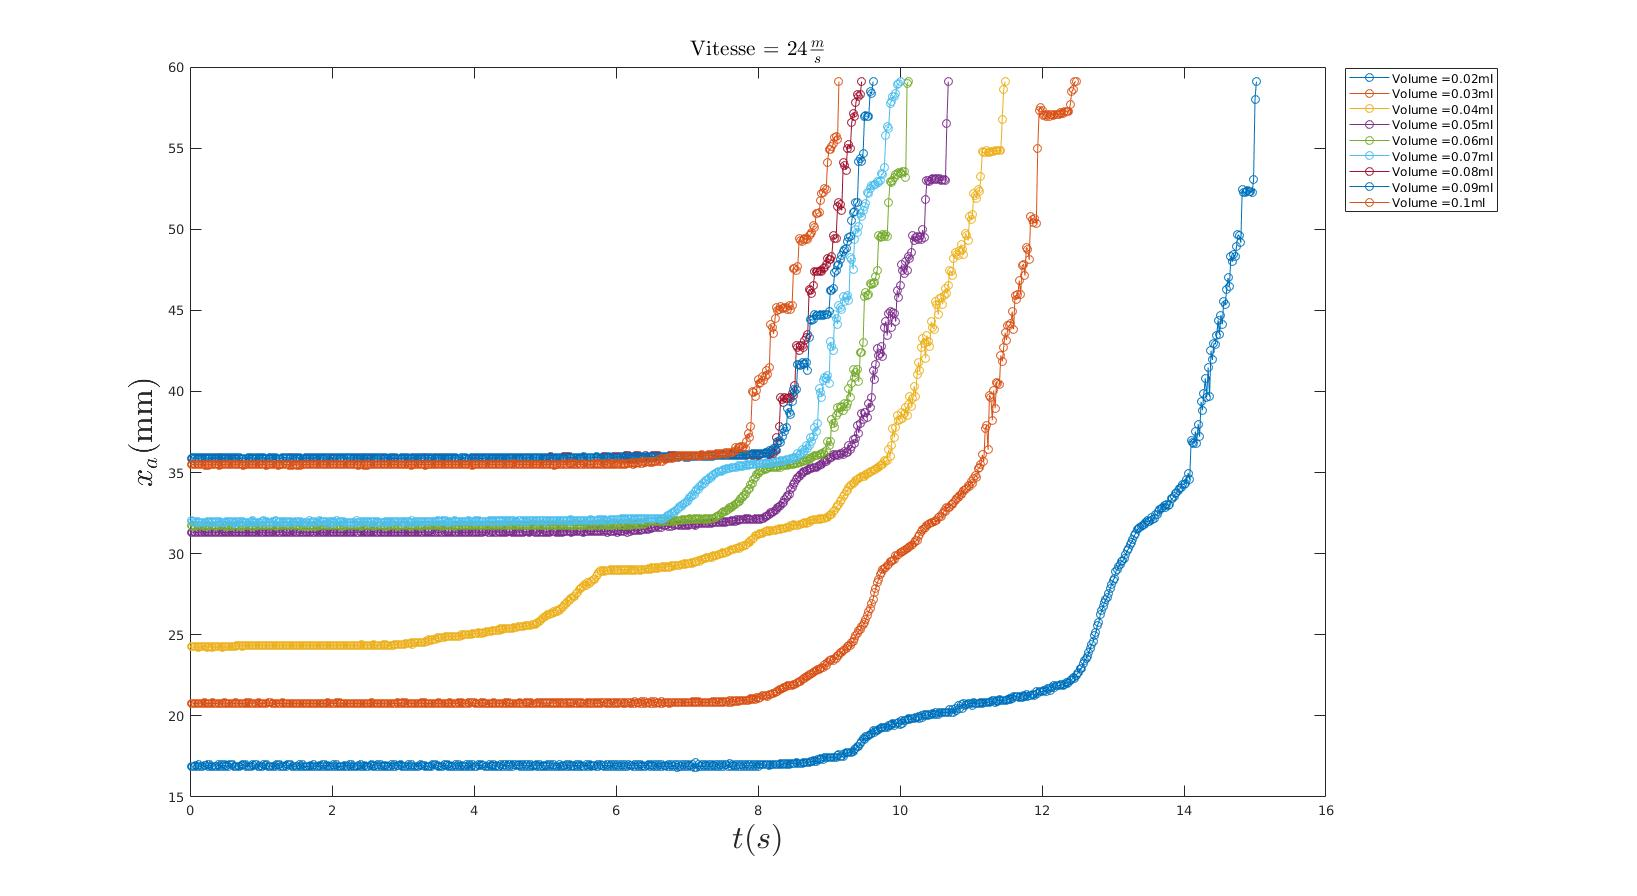
\includegraphics[width = \linewidth]{./image/v=24xa.jpg}
	\caption{Position à l'avant pour une vitesse de $24m\mathbin{/}s$}
\end{figure}
\begin{figure}[h]
	\centering
	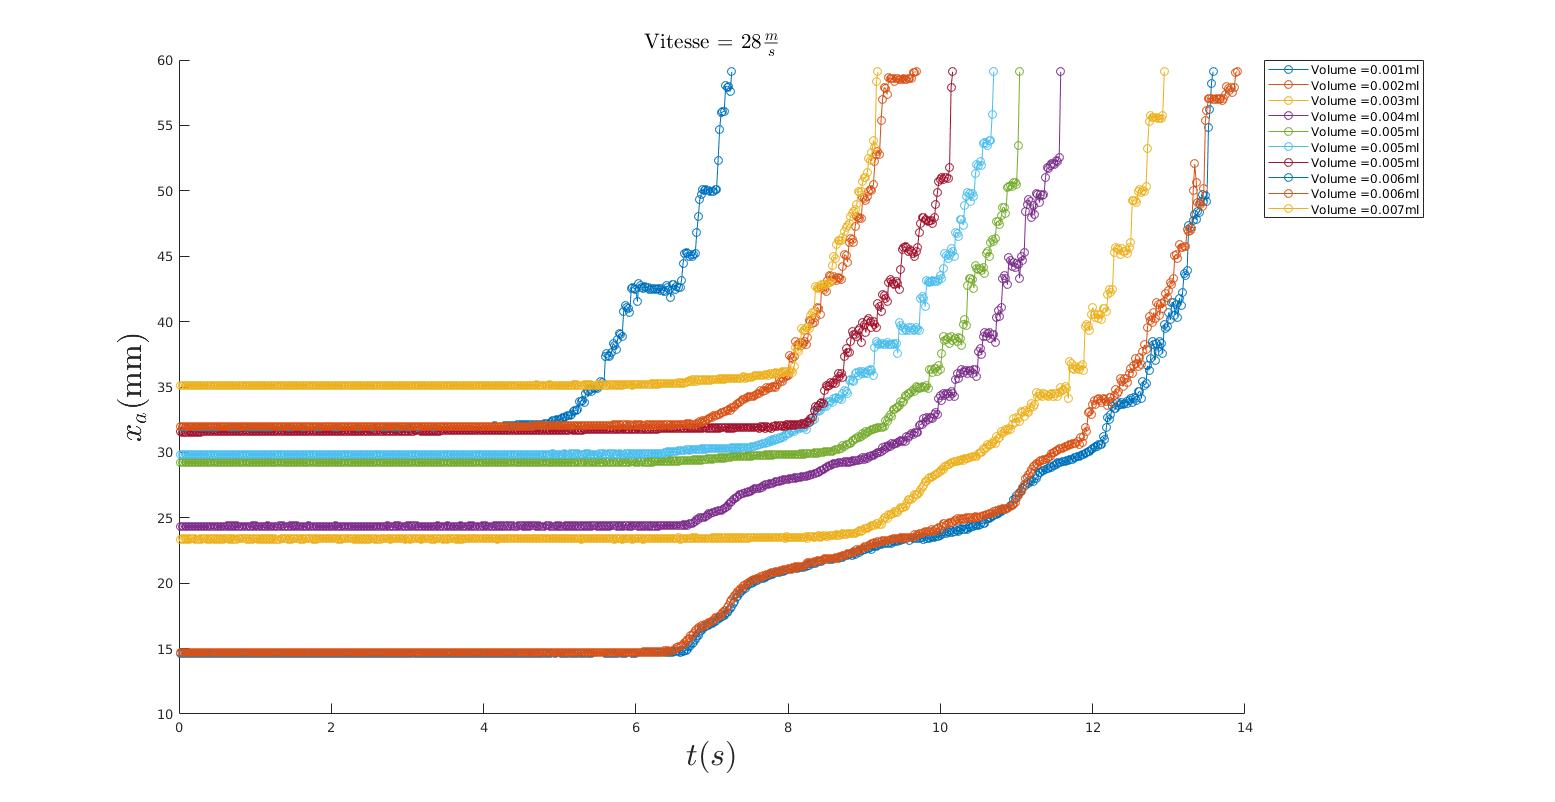
\includegraphics[width = \linewidth]{./image/v=28xa.jpg}
	\caption{Position à l'avant pour une vitesse de $28m\mathbin{/}s$}
\end{figure}

Nous a avions pu constater dans nos expériences que l'angle d'avancé augmentait globalement au cours du temps, ce que semble indiqué les figures.\\

Il y avait aussi des oscillations rapides autour d'un certaine position avant que la goutte avance de nouveau (le point avant avançait puis reculait) avant d'avant et c'est que doit traduire cette oscillation d'angle tout en augmentant globalement.

\newpage
\subsection{Position de l'arrière}
\begin{figure}[h]
	\centering
	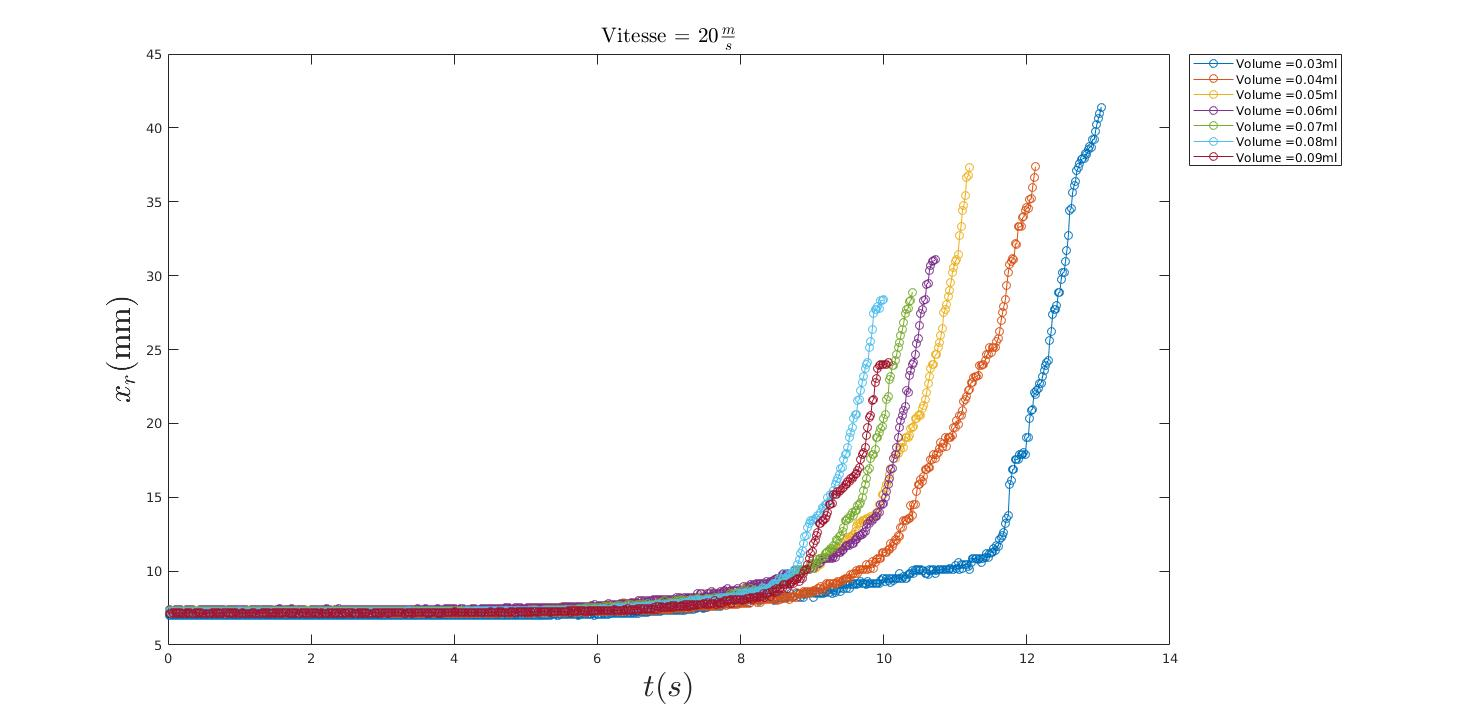
\includegraphics[width = \linewidth]{./image/v=20xr.jpg}
	\caption{Position à l'arrière pour une vitesse de $20m\mathbin{/}s$}
\end{figure}
\begin{figure}[h]
	\centering
	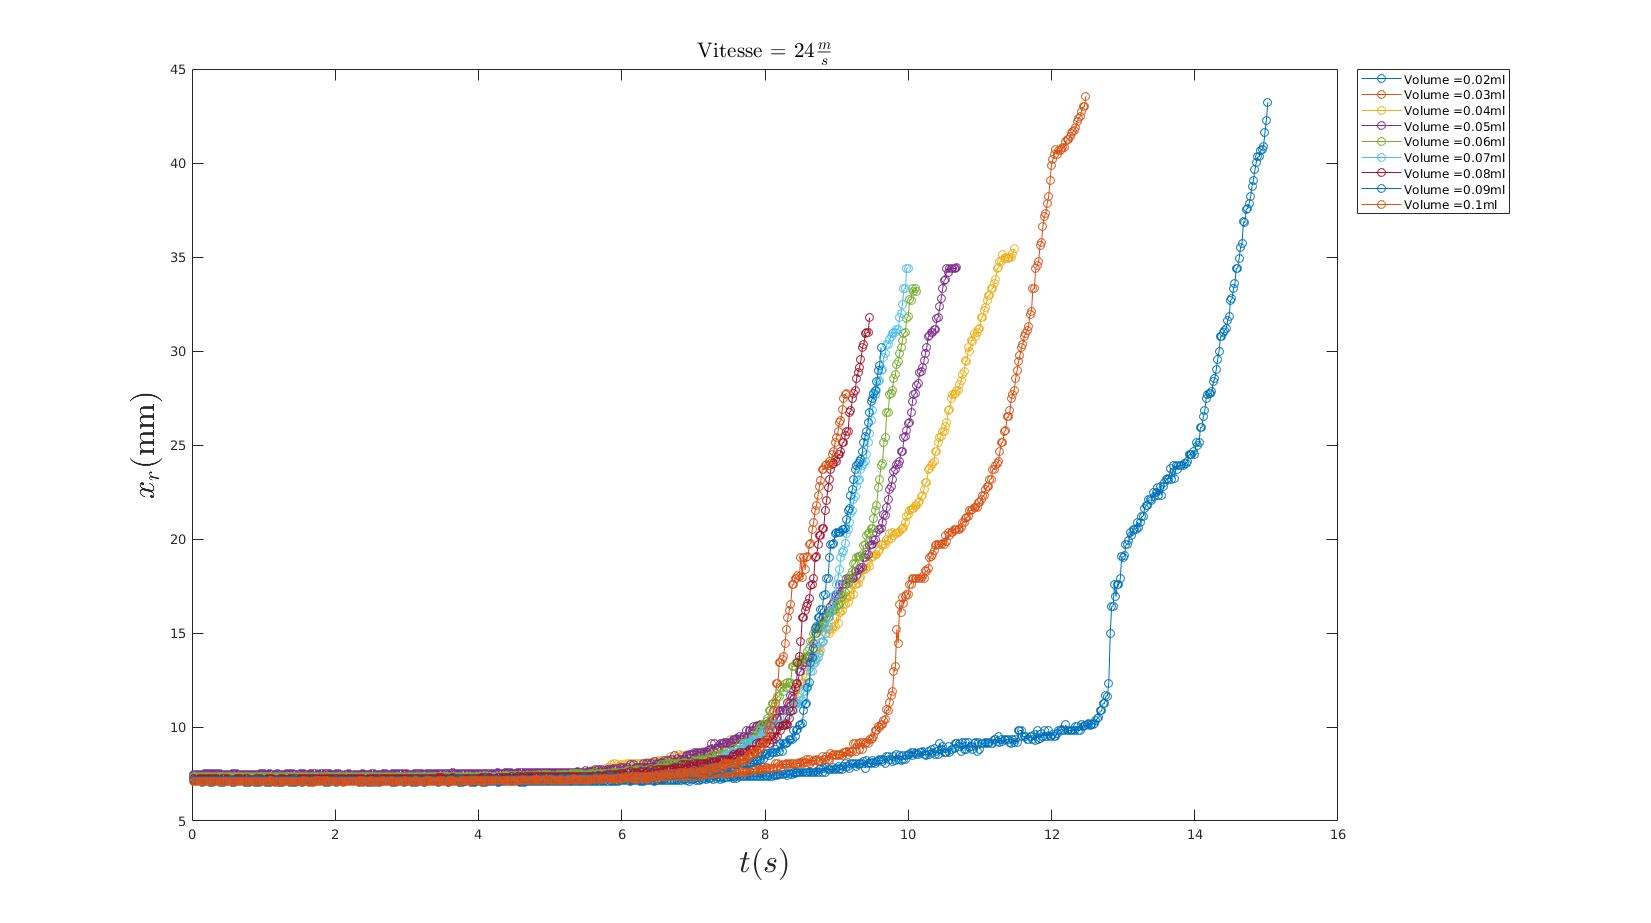
\includegraphics[width = \linewidth]{./image/v=24xr.jpg}
	\caption{Position à l'arrière pour une vitesse de $24m\mathbin{/}s$}
\end{figure}
\newpage
\begin{figure}[h]
	\centering
	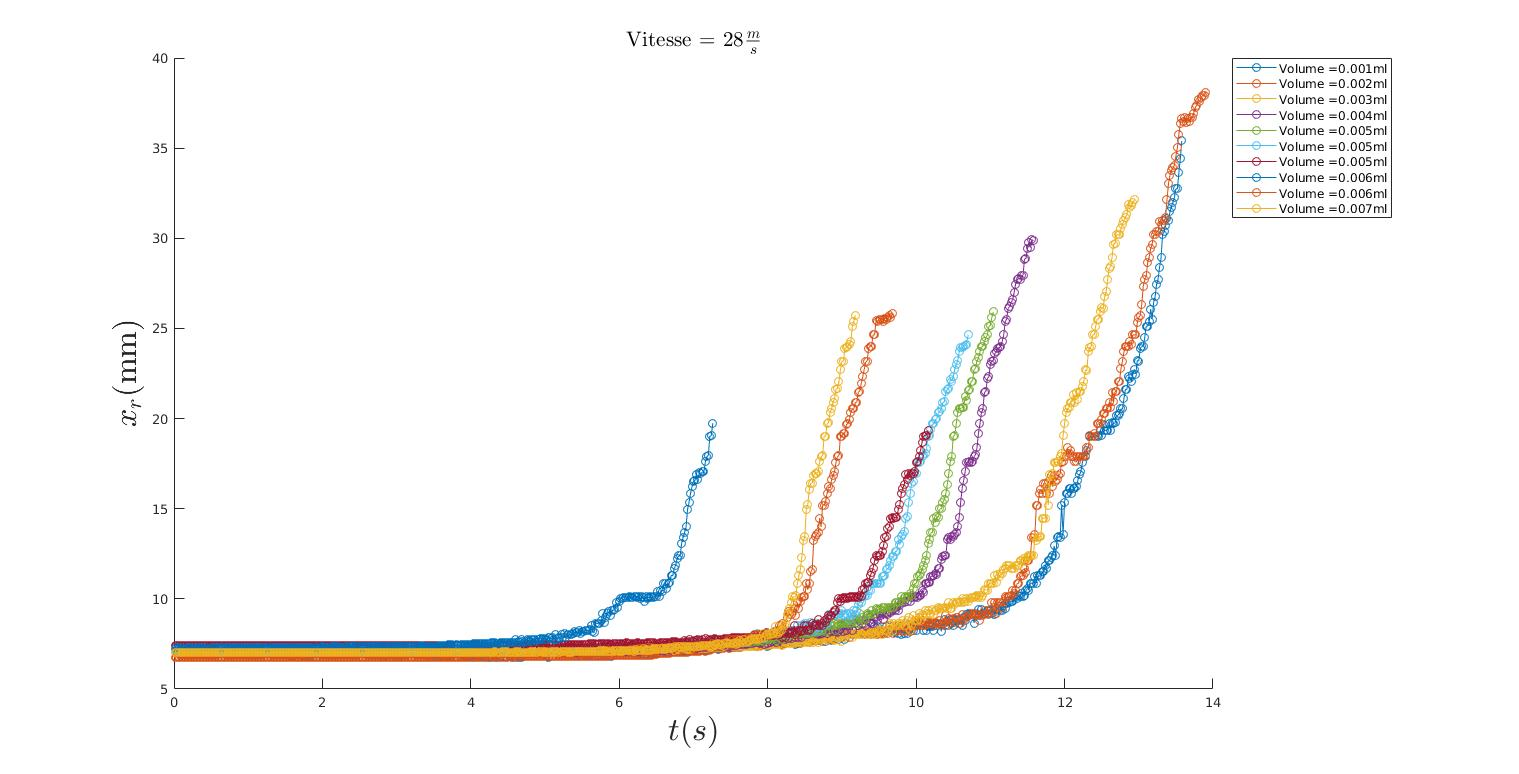
\includegraphics[width = \linewidth]{./image/v=28xr.jpg}
	\caption{Position à l'arrière pour une vitesse de $28m\mathbin{/}s$}
\end{figure}

Nous a avions pu constater dans nos expériences que l'angle d'avancé augmentait globalement au cours du temps, ce que semble indiqué les figures.\\

Il y avait aussi des oscillations rapides autour d'un certaine position arrière que la goutte avance de nouveau (le point arrière avançait puis reculait) arrière d'arrière et c'est que doit traduire cette oscillation d'angle tout en augmentant globalement.

\end{document}
